\setauthor{Moritz Eder}

\section{Mockups}

Als Grundlage für die Entwicklung des Design von Relaxoon standen Design-Mockups des Auftraggebers zur Verfügung.

\begin{figure}[H]
    \centering
    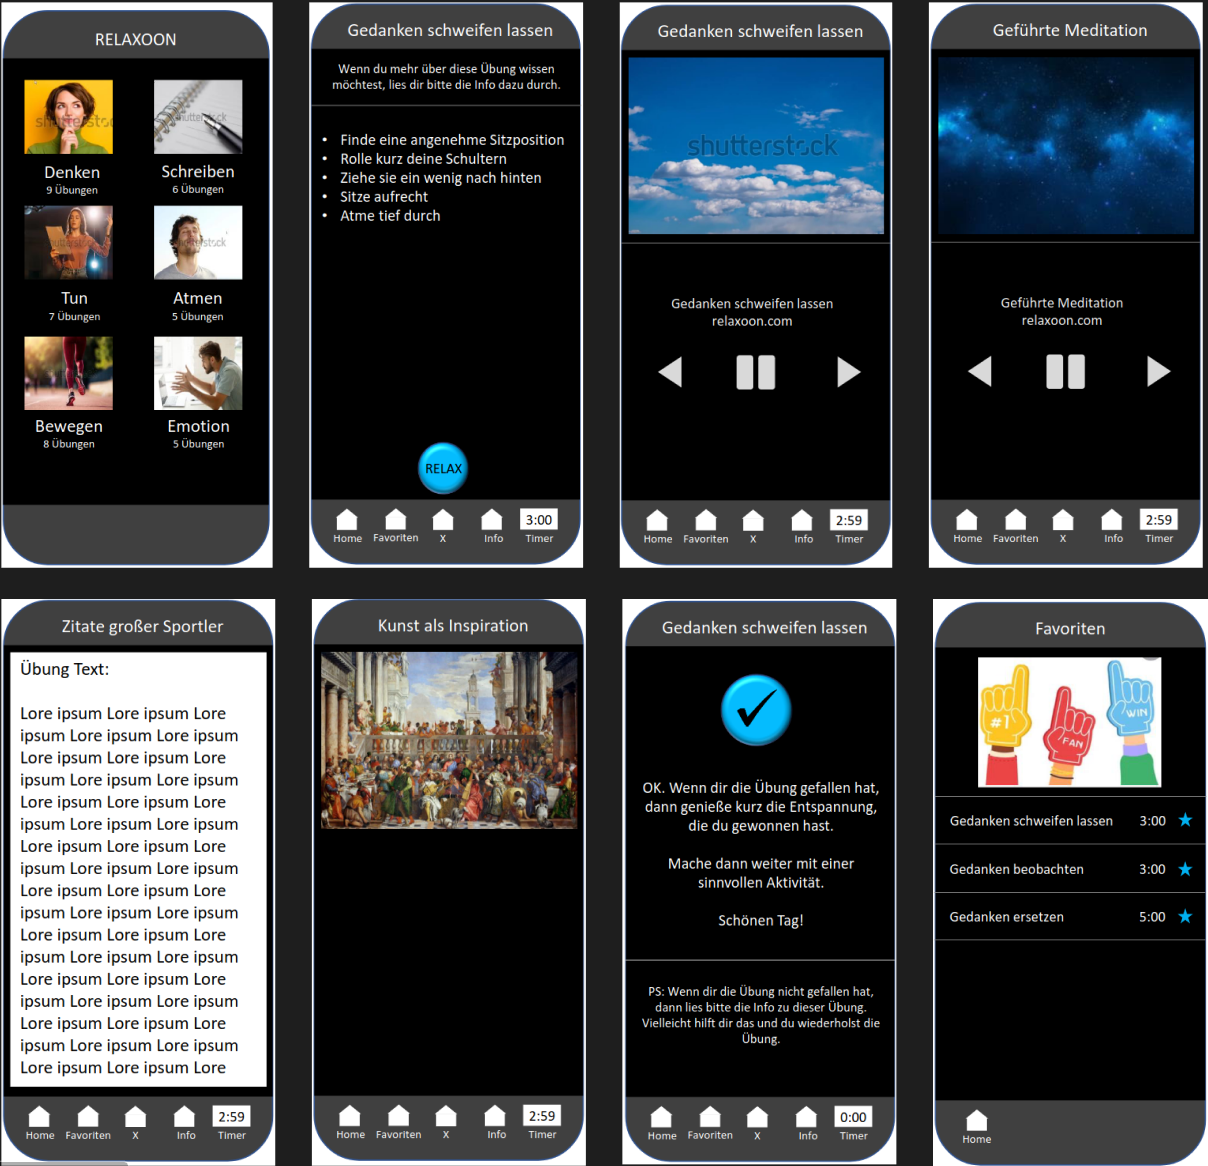
\includegraphics[height=\textwidth]{./pics/mockups.png}
    \caption{Mockups}
\end{figure}

Von oben links bis unten rechts auf dem Bild sind folgende Seiten abgebildet:

\begin{enumerate}
    \item Home-Screen
    \item Übung: Intro
    \item Übung: Video 
    \item Übung: Ton 
    \item Übung: Text 
    \item Übung: Foto 
    \item Übung: Outro
    \item Favoritenliste
\end{enumerate}

\section{Tutorial}

Zu Beginn, wenn man die App zum ersten Mal öffnet, kommt man zu einem Tutorial. Dieses gibt den User:innen einen ersten
Einblick in die App.

Im UI-Prototypen von Relaxoon wurde das Tutorial folgendermaßen realisiert:

\begin{figure}[H]
    \centering
    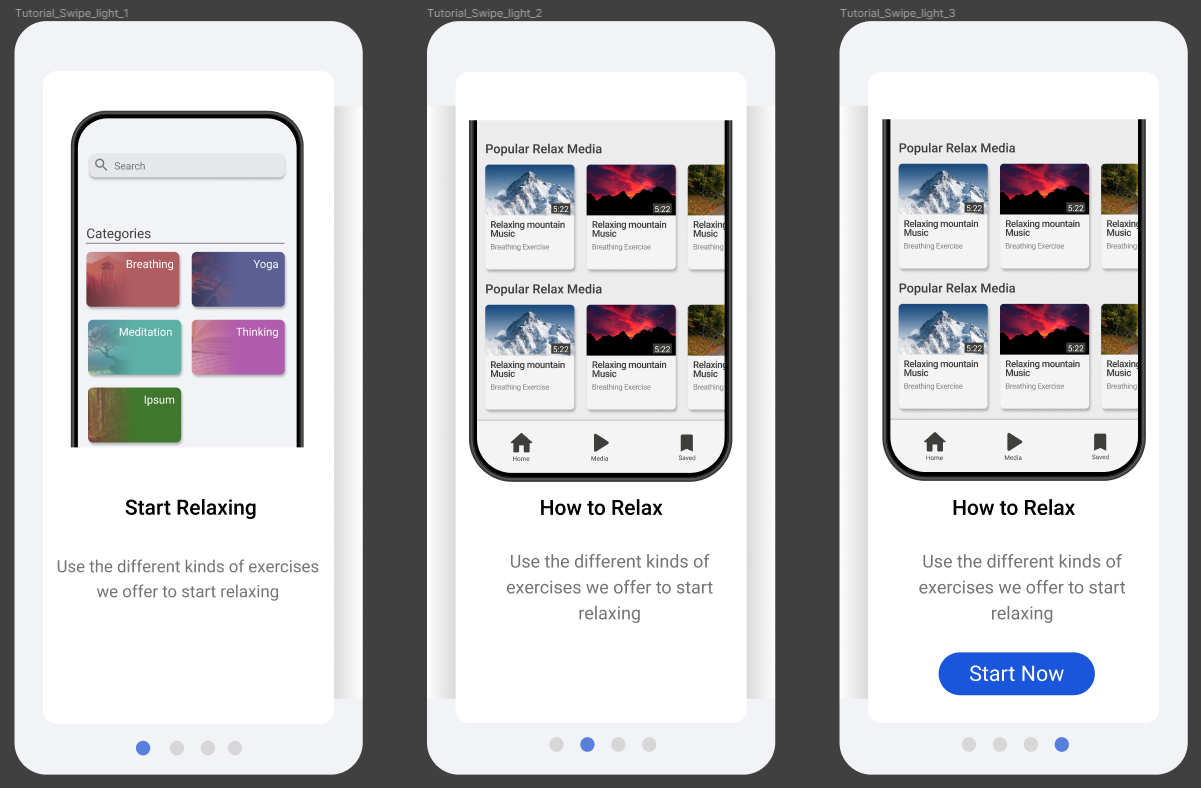
\includegraphics[height=0.65\textwidth]{./pics/pTutorial.png}
    \caption{Tutorial im UI-Prototypen}
\end{figure}

\newpage

Das Konzept wurde bei der Programmierung wie folgt verwirklicht:

\begin{figure}[H]
    \centering
    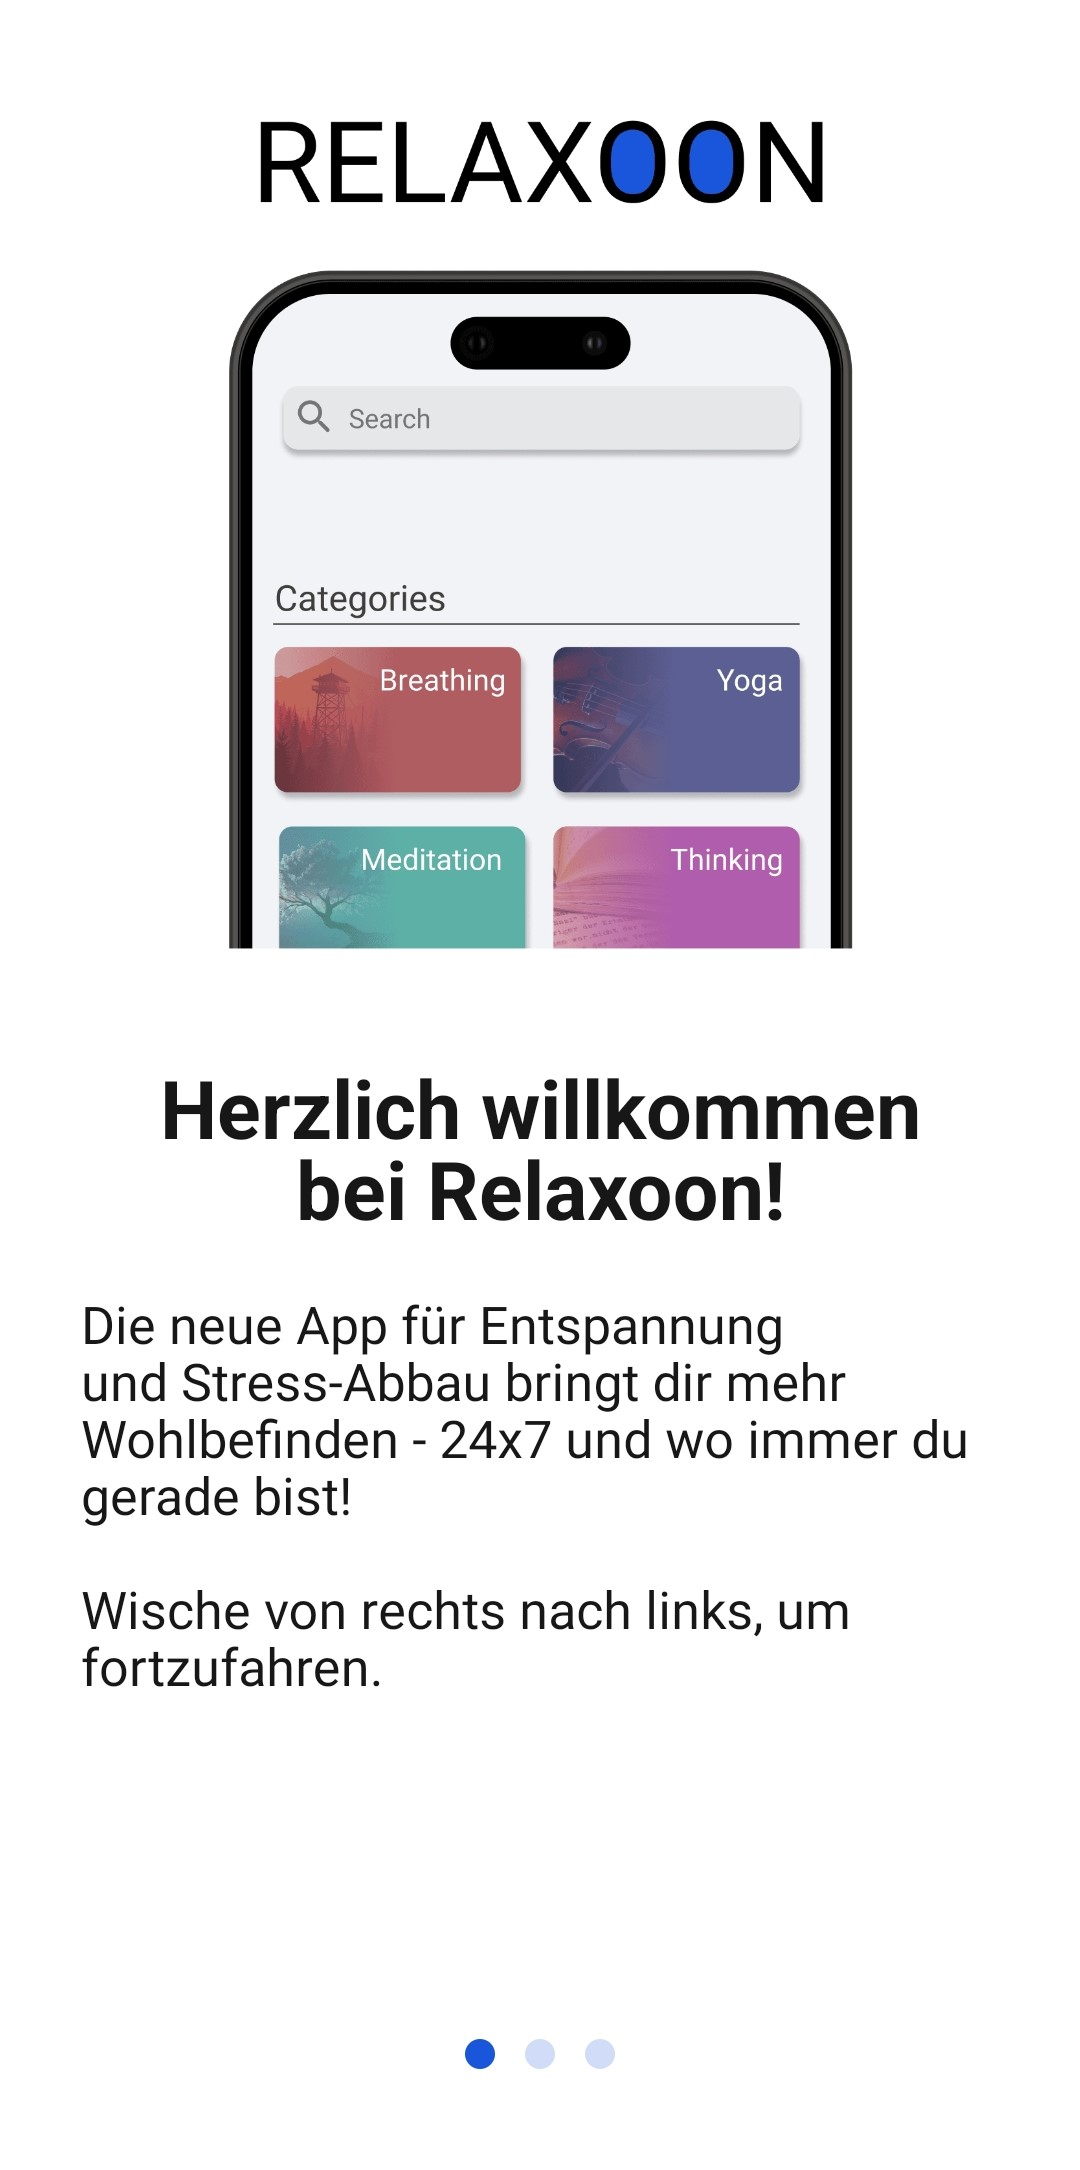
\includegraphics[height=0.71\textwidth]{./pics/Tutorial1.jpg}
    \caption{Erste Tutorial-Page}
\end{figure}
\begin{figure}[H]
    \centering
    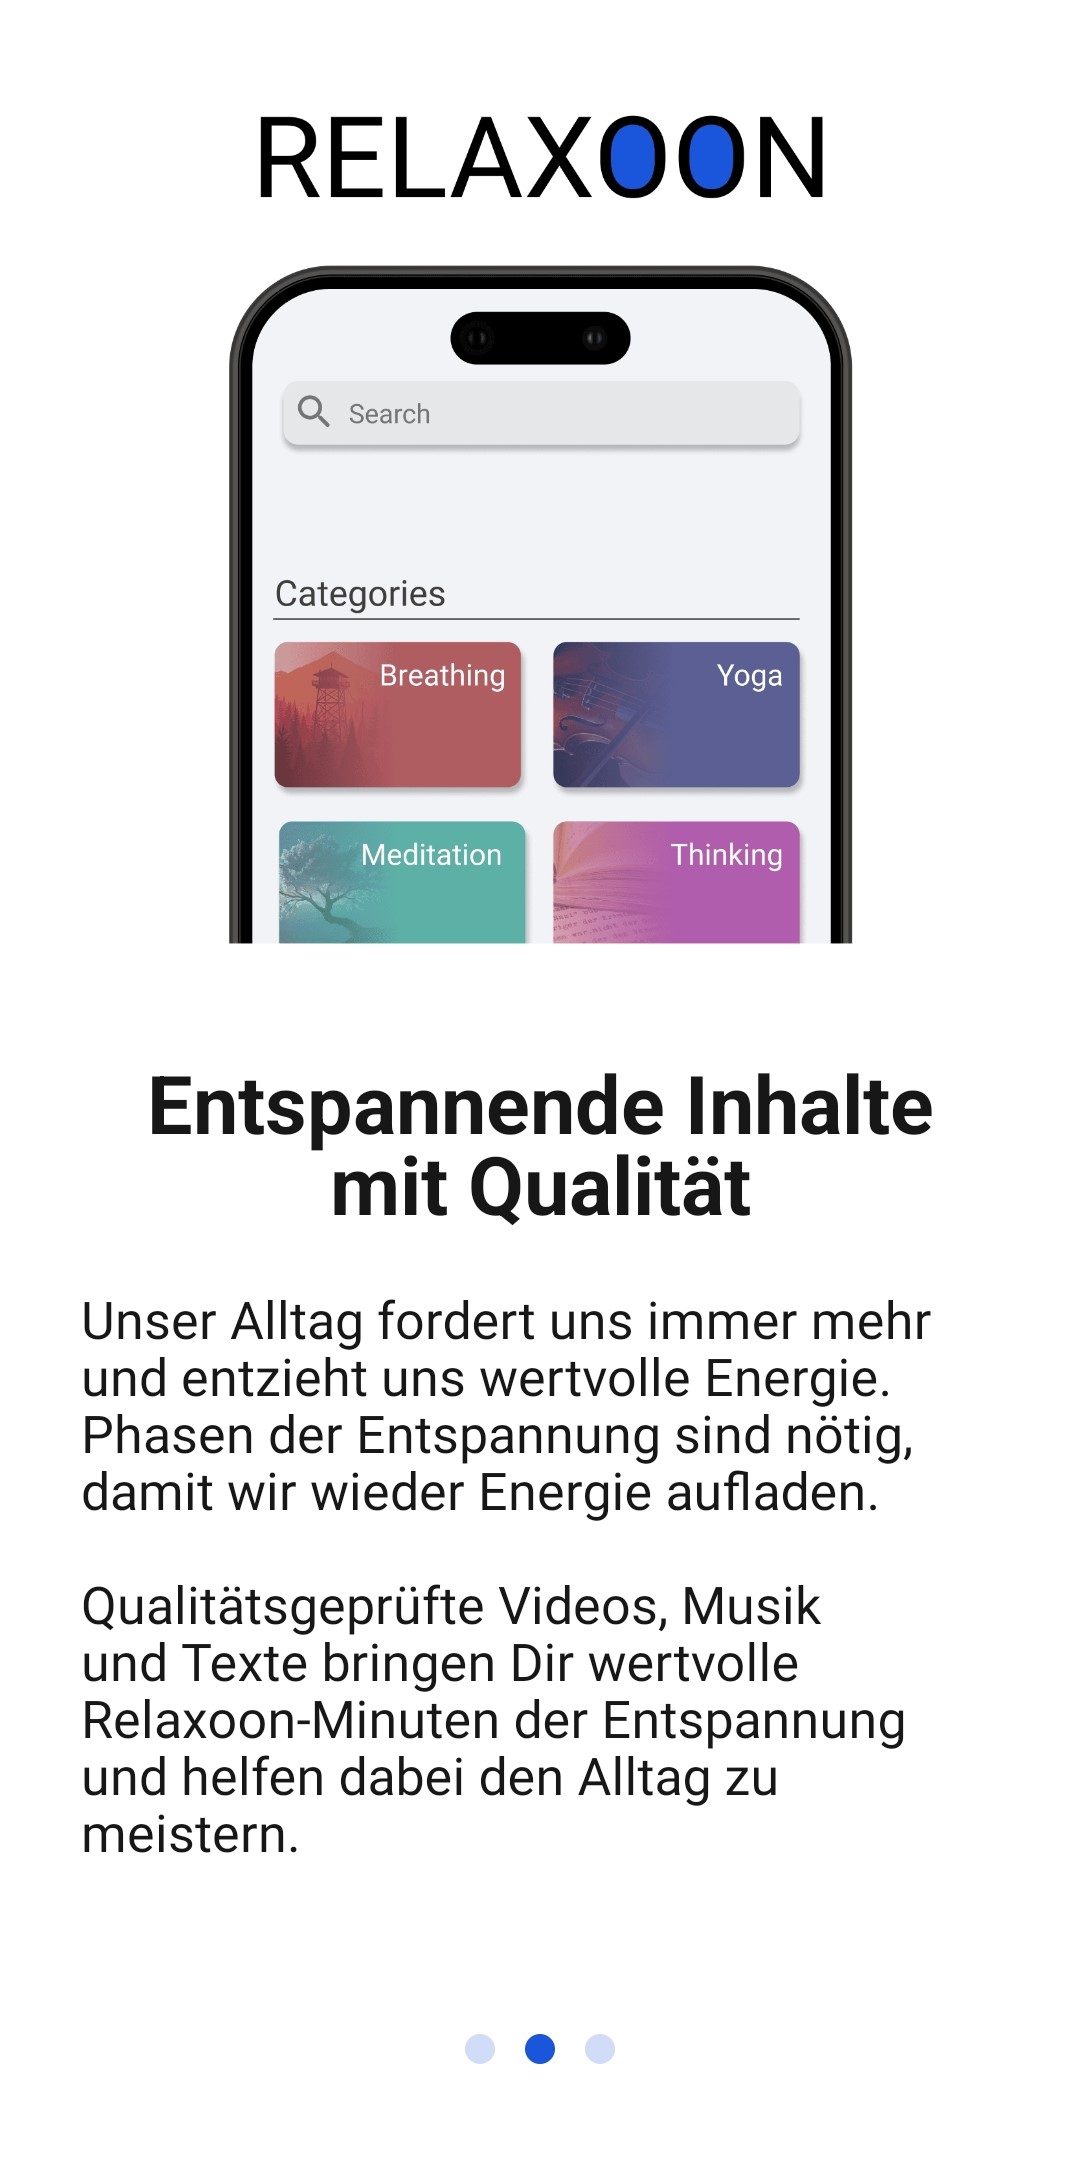
\includegraphics[height=0.71\textwidth]{./pics/Tutorial2.jpg}
    \caption{Zweite Tutorial-Page}
\end{figure}
\begin{figure}[H]
    \centering
    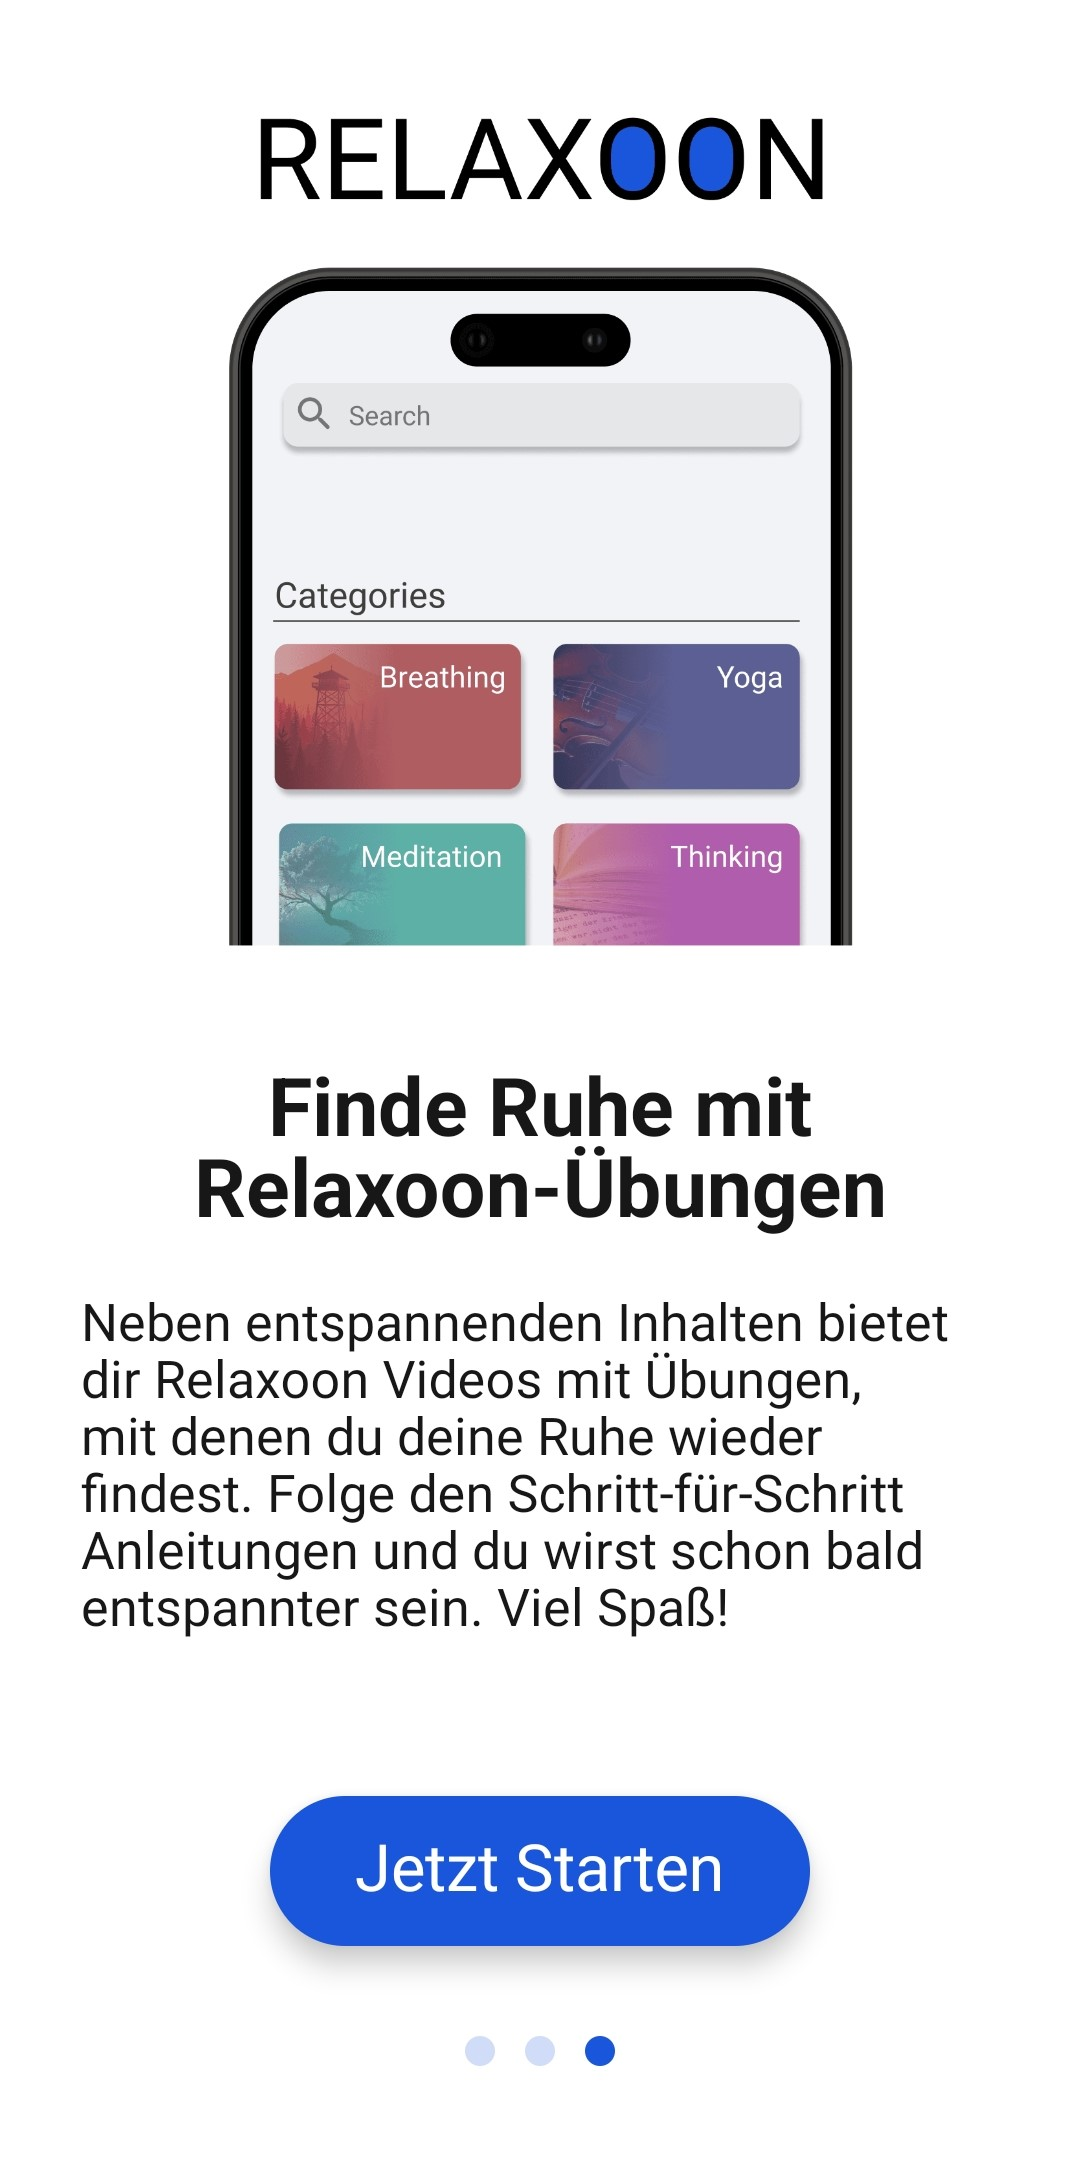
\includegraphics[height=\textwidth]{./pics/Tutorial3.jpg}
    \caption{Dritte Tutorial-Page}
\end{figure}

Auf der letzten Tutorial-Page gelangt man über den ''Jetzt Starten''-Button weiter zum Registrierungsformular.

\section{Login- und Registrierungsformular}

Das Registrierungsformular ist, wie unten dargestellt, nach folgendem Schema aufgebaut:

\begin{enumerate}
    \item Username
    \item E-Mail 
    \item Passwort 
    \item Passwort erneut eingeben
\end{enumerate}

\begin{figure}[H]
    \begin{minipage}{0.5\textwidth}
        \centering
        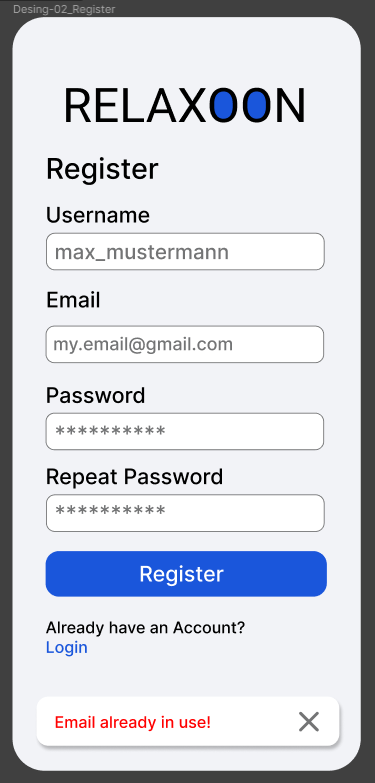
\includegraphics[height=2\textwidth]{./pics/pRegister.png}
        \caption{Registrierung UI-Prototyp}
    \end{minipage}
    \begin{minipage}{0.5\textwidth}
        \centering
        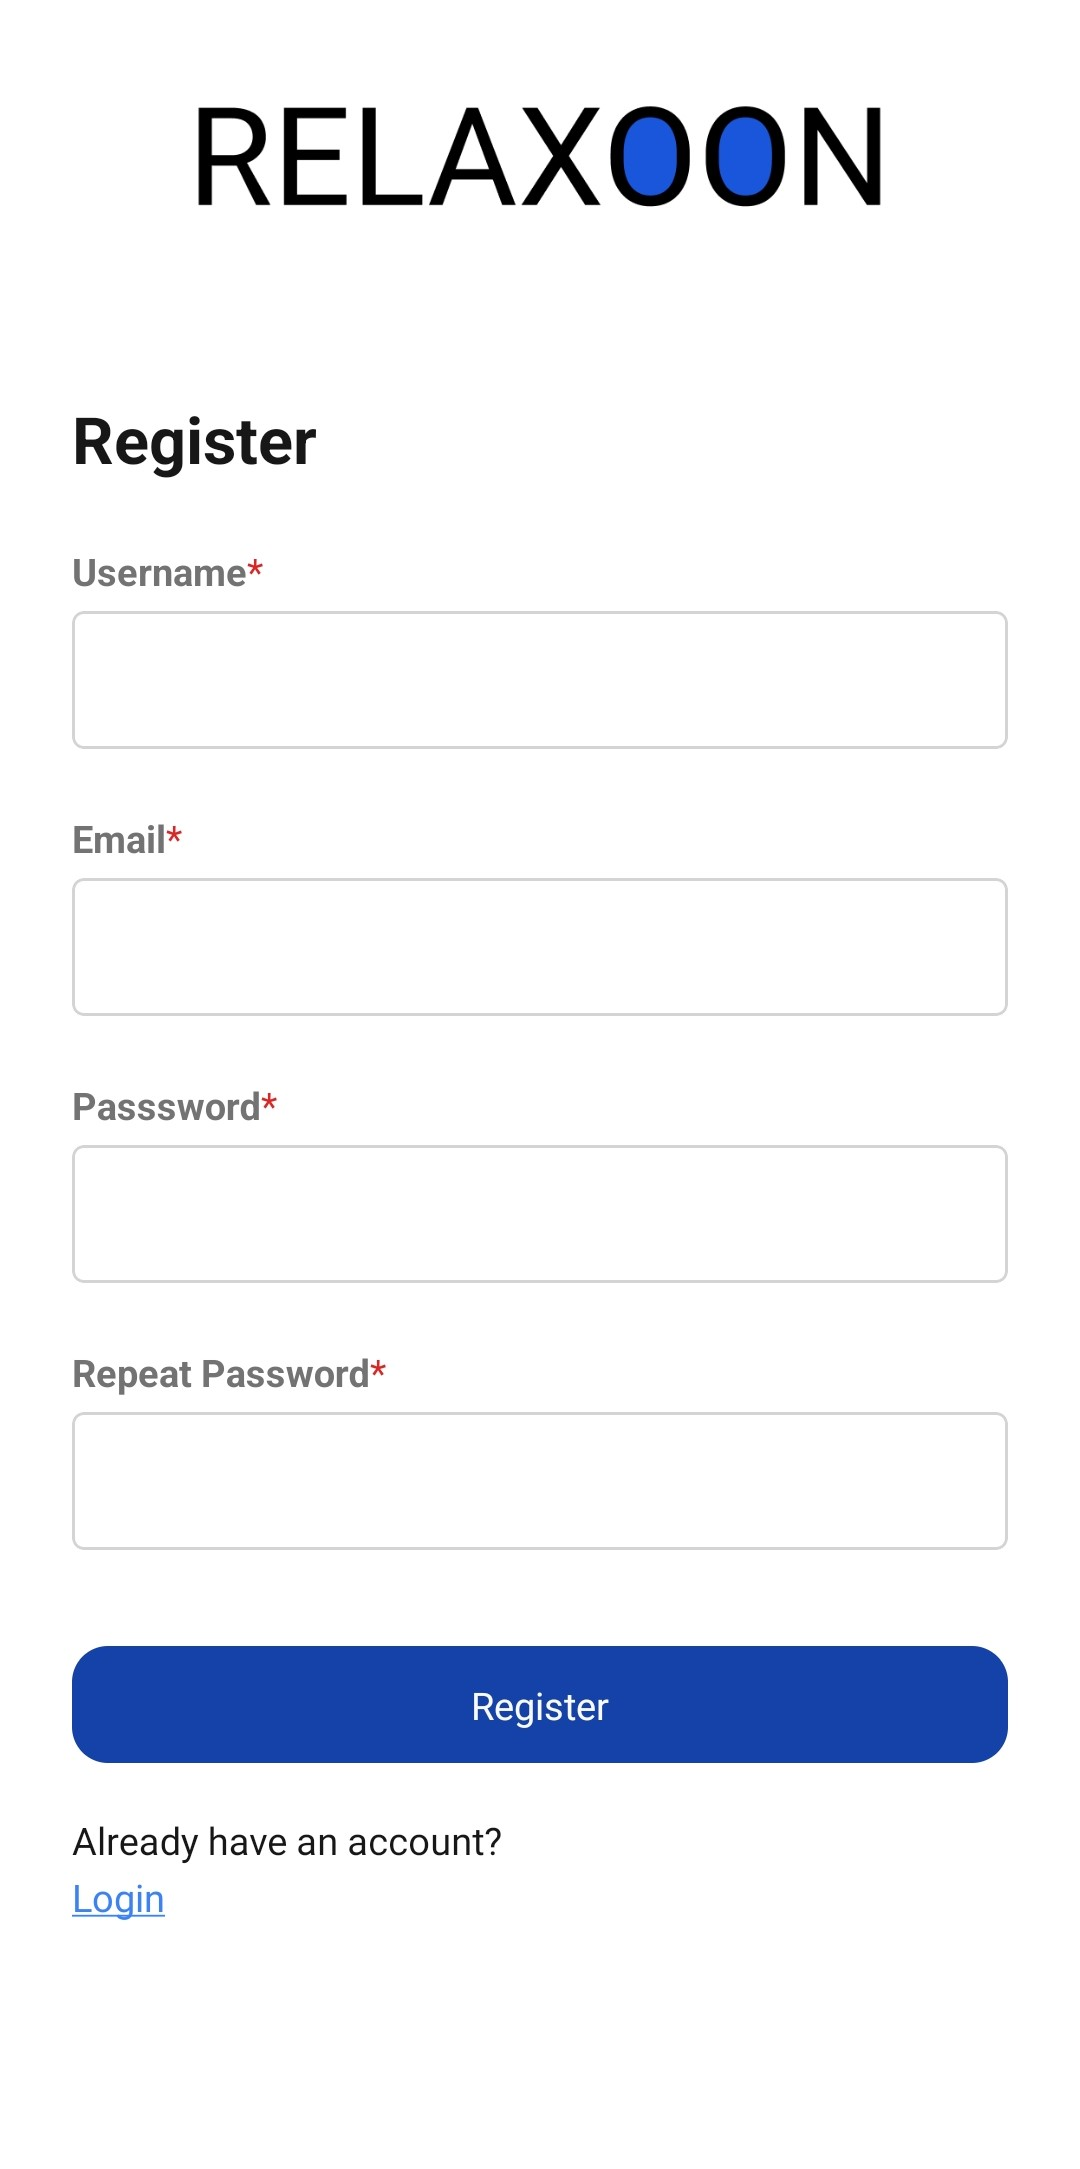
\includegraphics[height=2\textwidth]{./pics/register.jpg}
        \caption{Registrierung in der App}
    \end{minipage}
\end{figure}

Mit dem ''Register''-Button kommt man zum Home-Screen, sofern der Username, die E-Mail und das Passwort korrekt validiert
werden können.

Falls man bereits einen Account besitzt, kann man über das blaue ''Login'' zum Login-Screen navigieren.

\newpage

Um sich einloggen zu können, muss man bei diesem Screen die bereits registrierte E-Mail und das dazugehörige Passwort 
eingeben und auf ''Login'' drücken. Damit gelangt man ebenfalls zum Home-Screen. Über das blaue ''Create an Account''
wird man zurück zur Registrierung geleitet, falls man sich einen neuen Account erstellen will.

\begin{figure}[H]
    \begin{minipage}{0.5\textwidth}
        \centering
        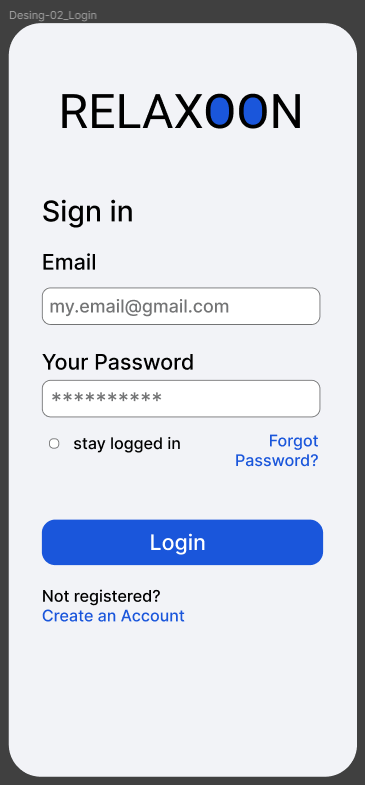
\includegraphics[height=2\textwidth]{./pics/pLogin.png}
        \caption{Login UI-Prototyp}
    \end{minipage}
    \begin{minipage}{0.5\textwidth}
        \centering
        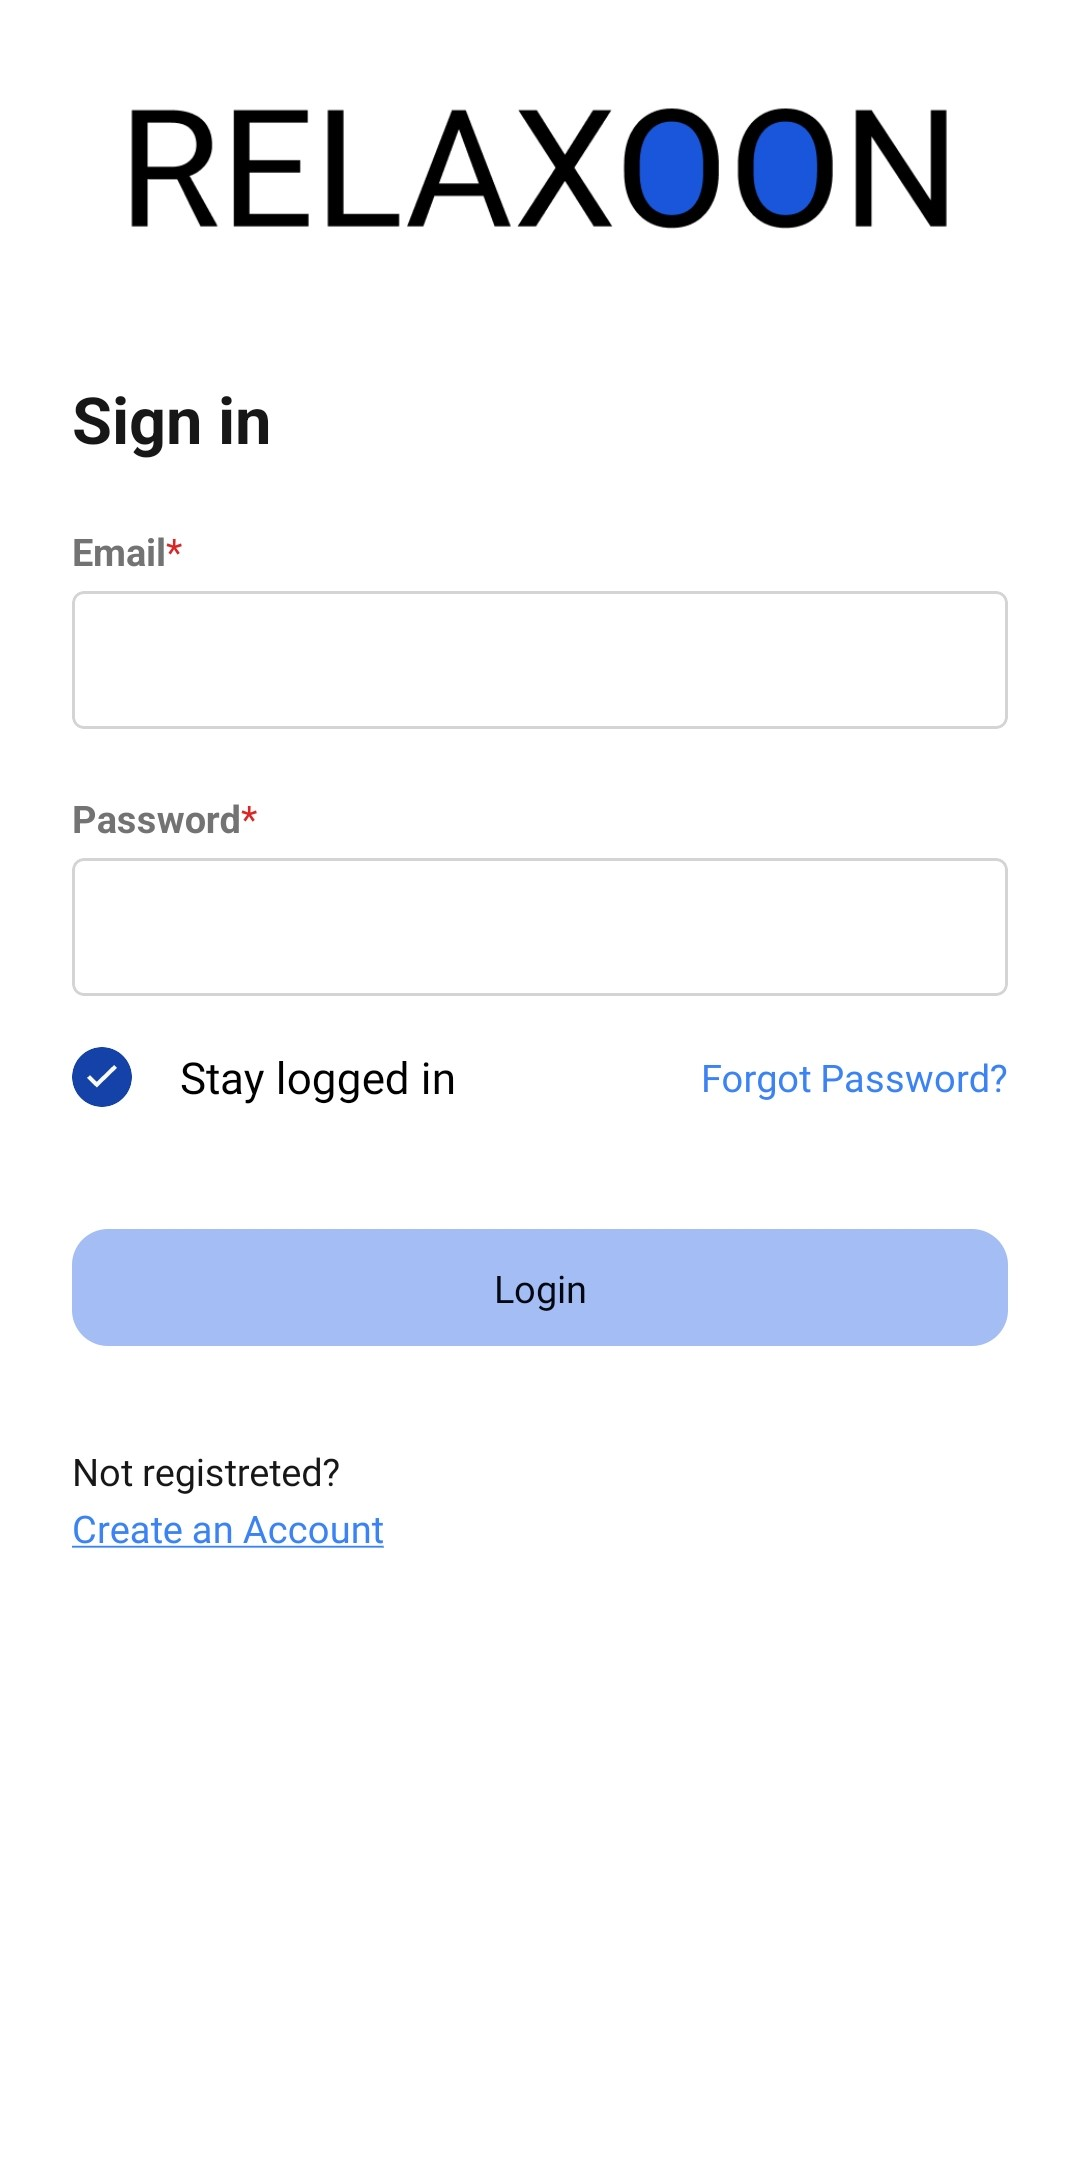
\includegraphics[height=2\textwidth]{./pics/login.jpg}
        \caption{Login in der App}
    \end{minipage}
\end{figure}

Bei erfolgreichem Login wird der/die User:in darüber mit einer Nachricht informiert, die am unteren des Bildschirms 
aufscheint.

\begin{figure}[H]
    \centering
    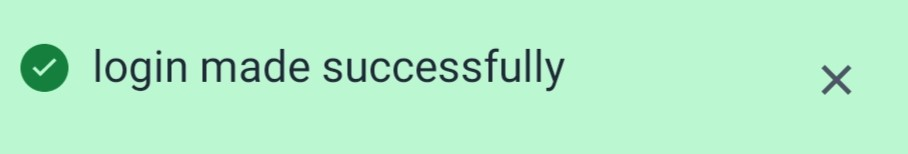
\includegraphics[height=0.09\textwidth]{./pics/message_cut.jpg}
    \caption{Bestätigungsnachricht}
\end{figure}

\section{Home-Screen}

\begin{figure}[H]
    \centering
    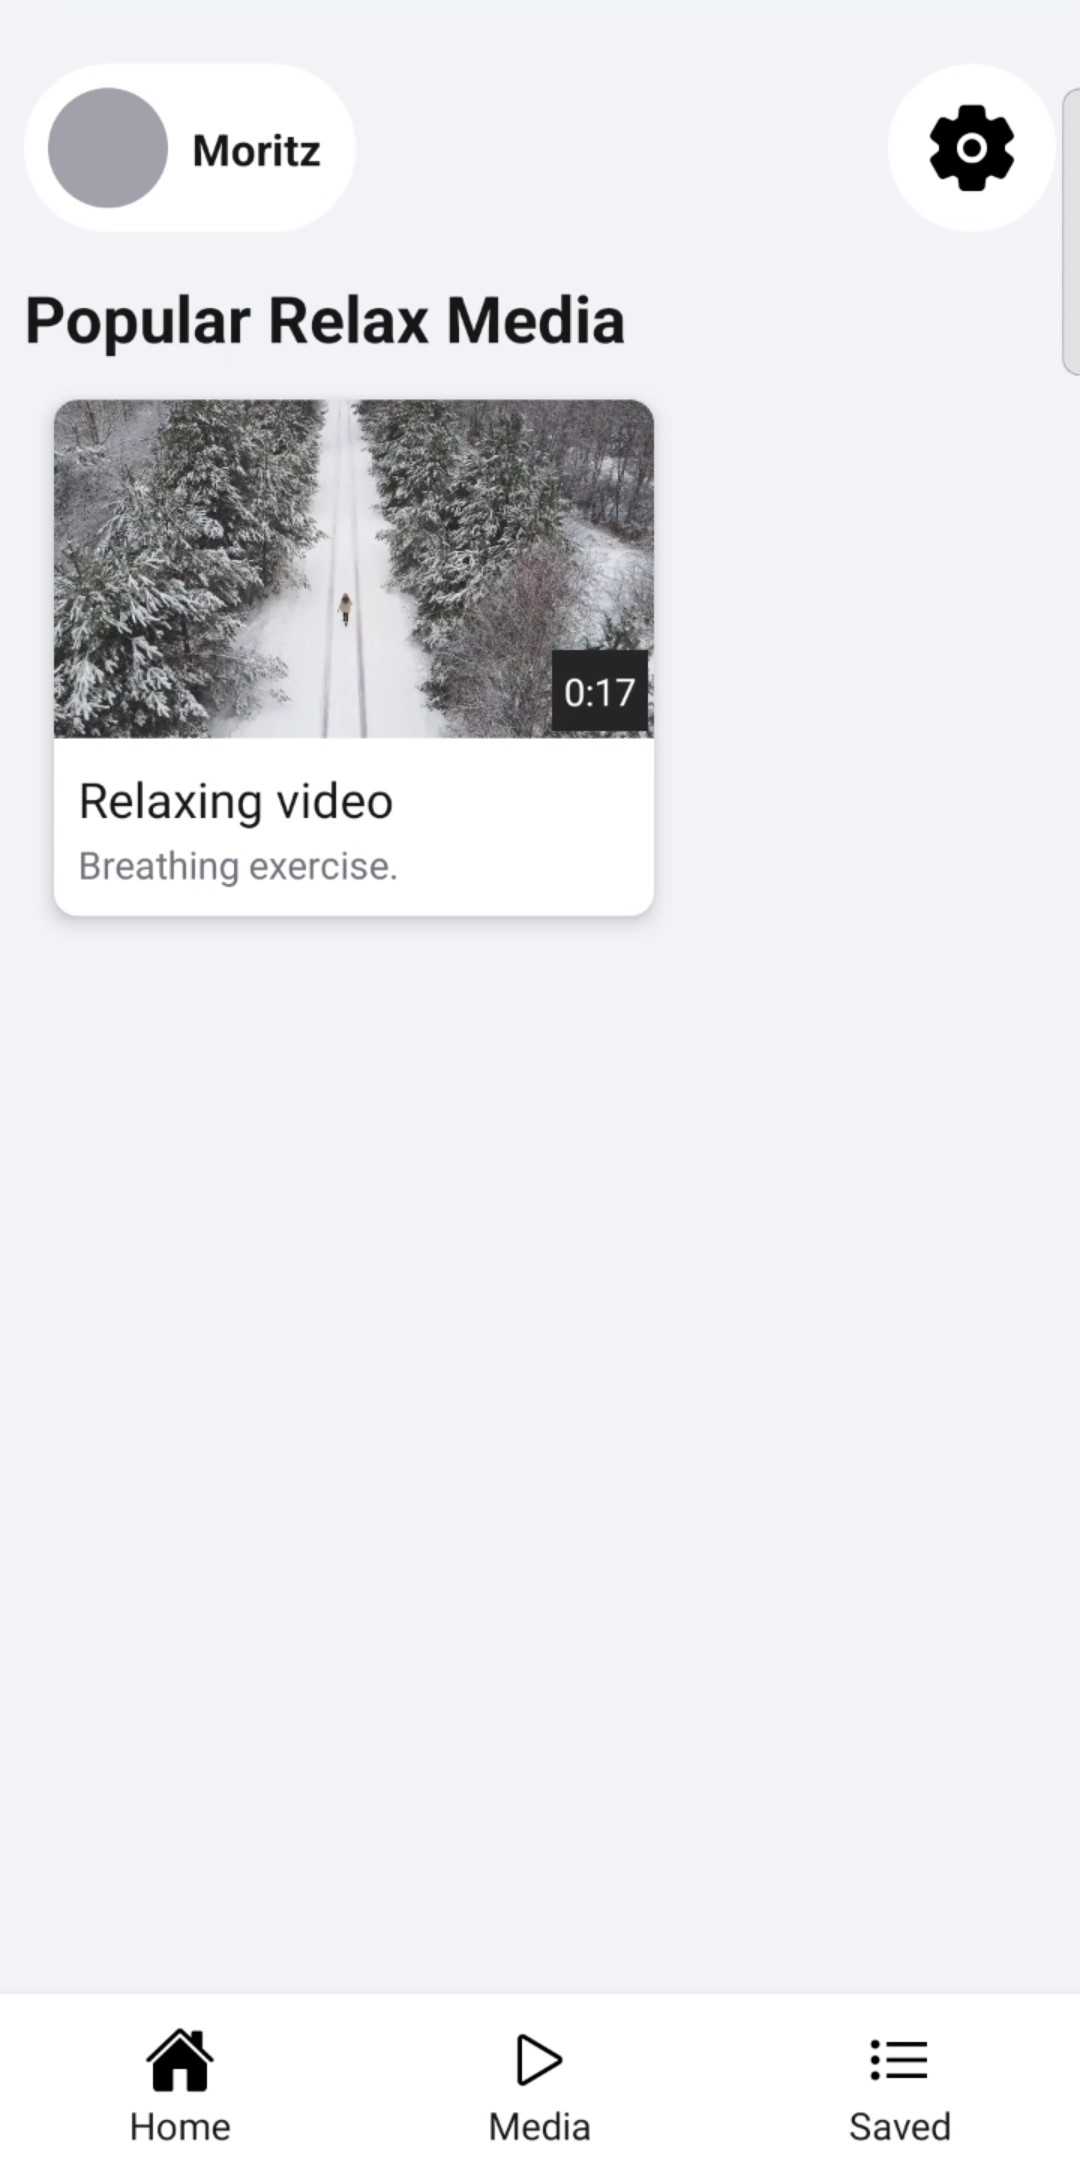
\includegraphics[height=\textwidth]{./pics/Home.jpg}
    \caption{Home-Screen}
\end{figure}

\section{Kategorien}

\begin{figure}[H]
    \begin{minipage}{0.5\textwidth}
        \centering
        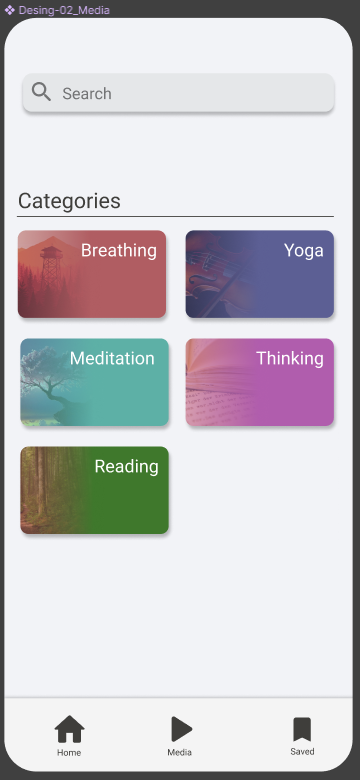
\includegraphics[height=2\textwidth]{./pics/pKategorien.png}
        \caption{Kategorien UI-Prototyp}
    \end{minipage}
    \begin{minipage}{0.5\textwidth}
        \centering
        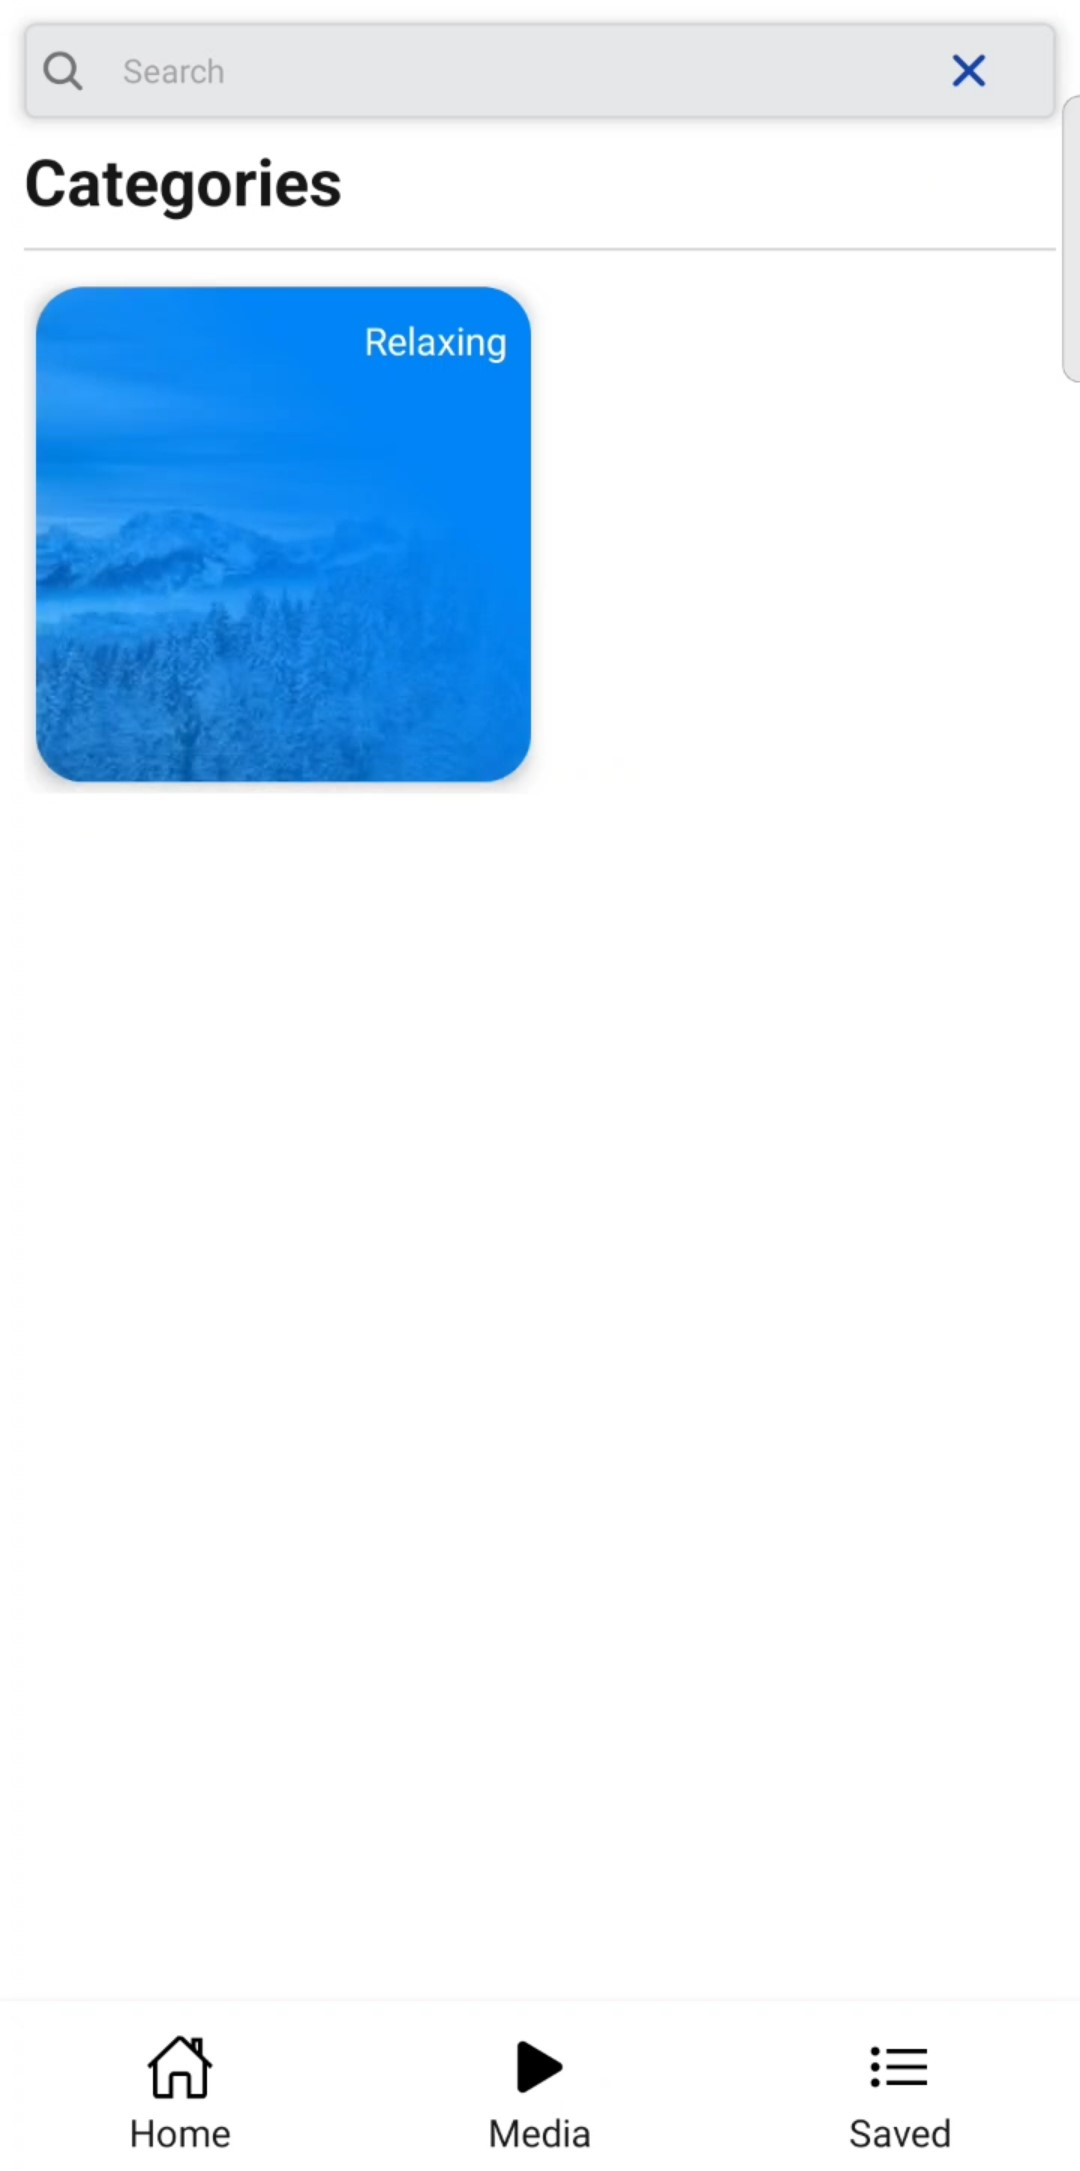
\includegraphics[height=2\textwidth]{./pics/Kategorien.jpg}
        \caption{Kategorien in der App}
    \end{minipage}
\end{figure}

\begin{figure}[H]
    \begin{minipage}{0.5\textwidth}
        \centering
        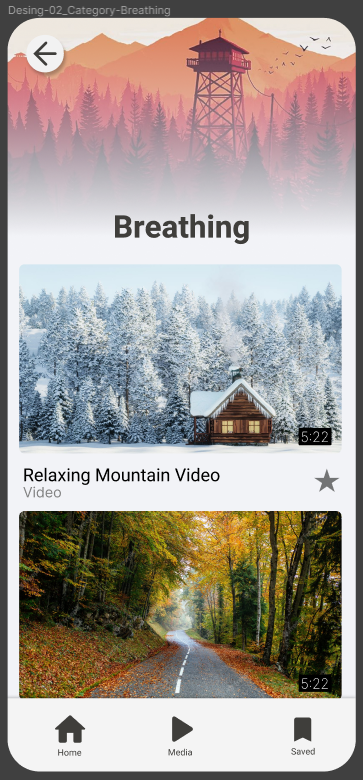
\includegraphics[height=2\textwidth]{./pics/pKategorie.png}
        \caption{Kategorien UI-Prototyp}
    \end{minipage}
    \begin{minipage}{0.5\textwidth}
        \centering
        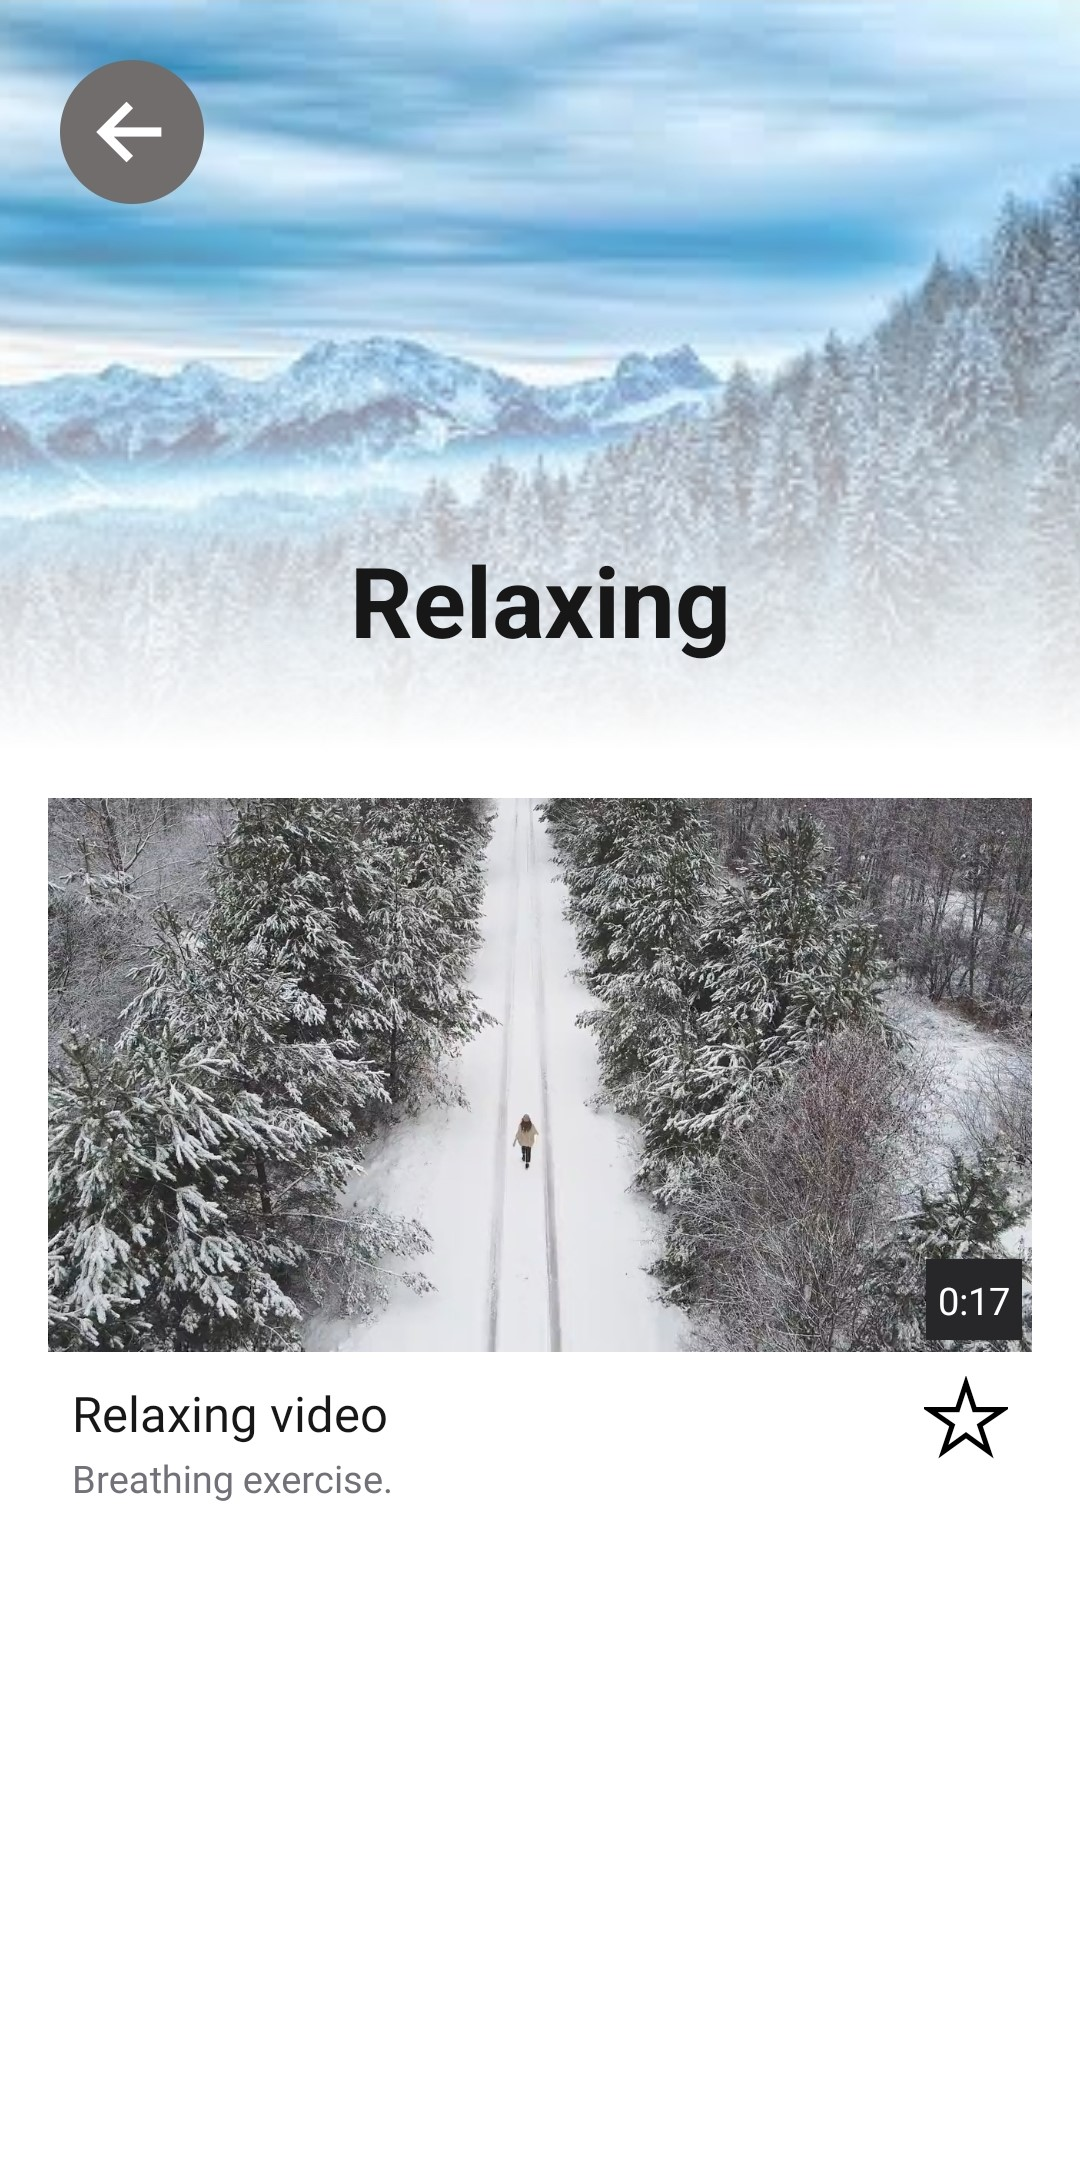
\includegraphics[height=2\textwidth]{./pics/Kategorie.jpg}
        \caption{Kategorie in der App}
    \end{minipage}
\end{figure}

\section{Suchleiste}

\begin{figure}[H]
    \centering
    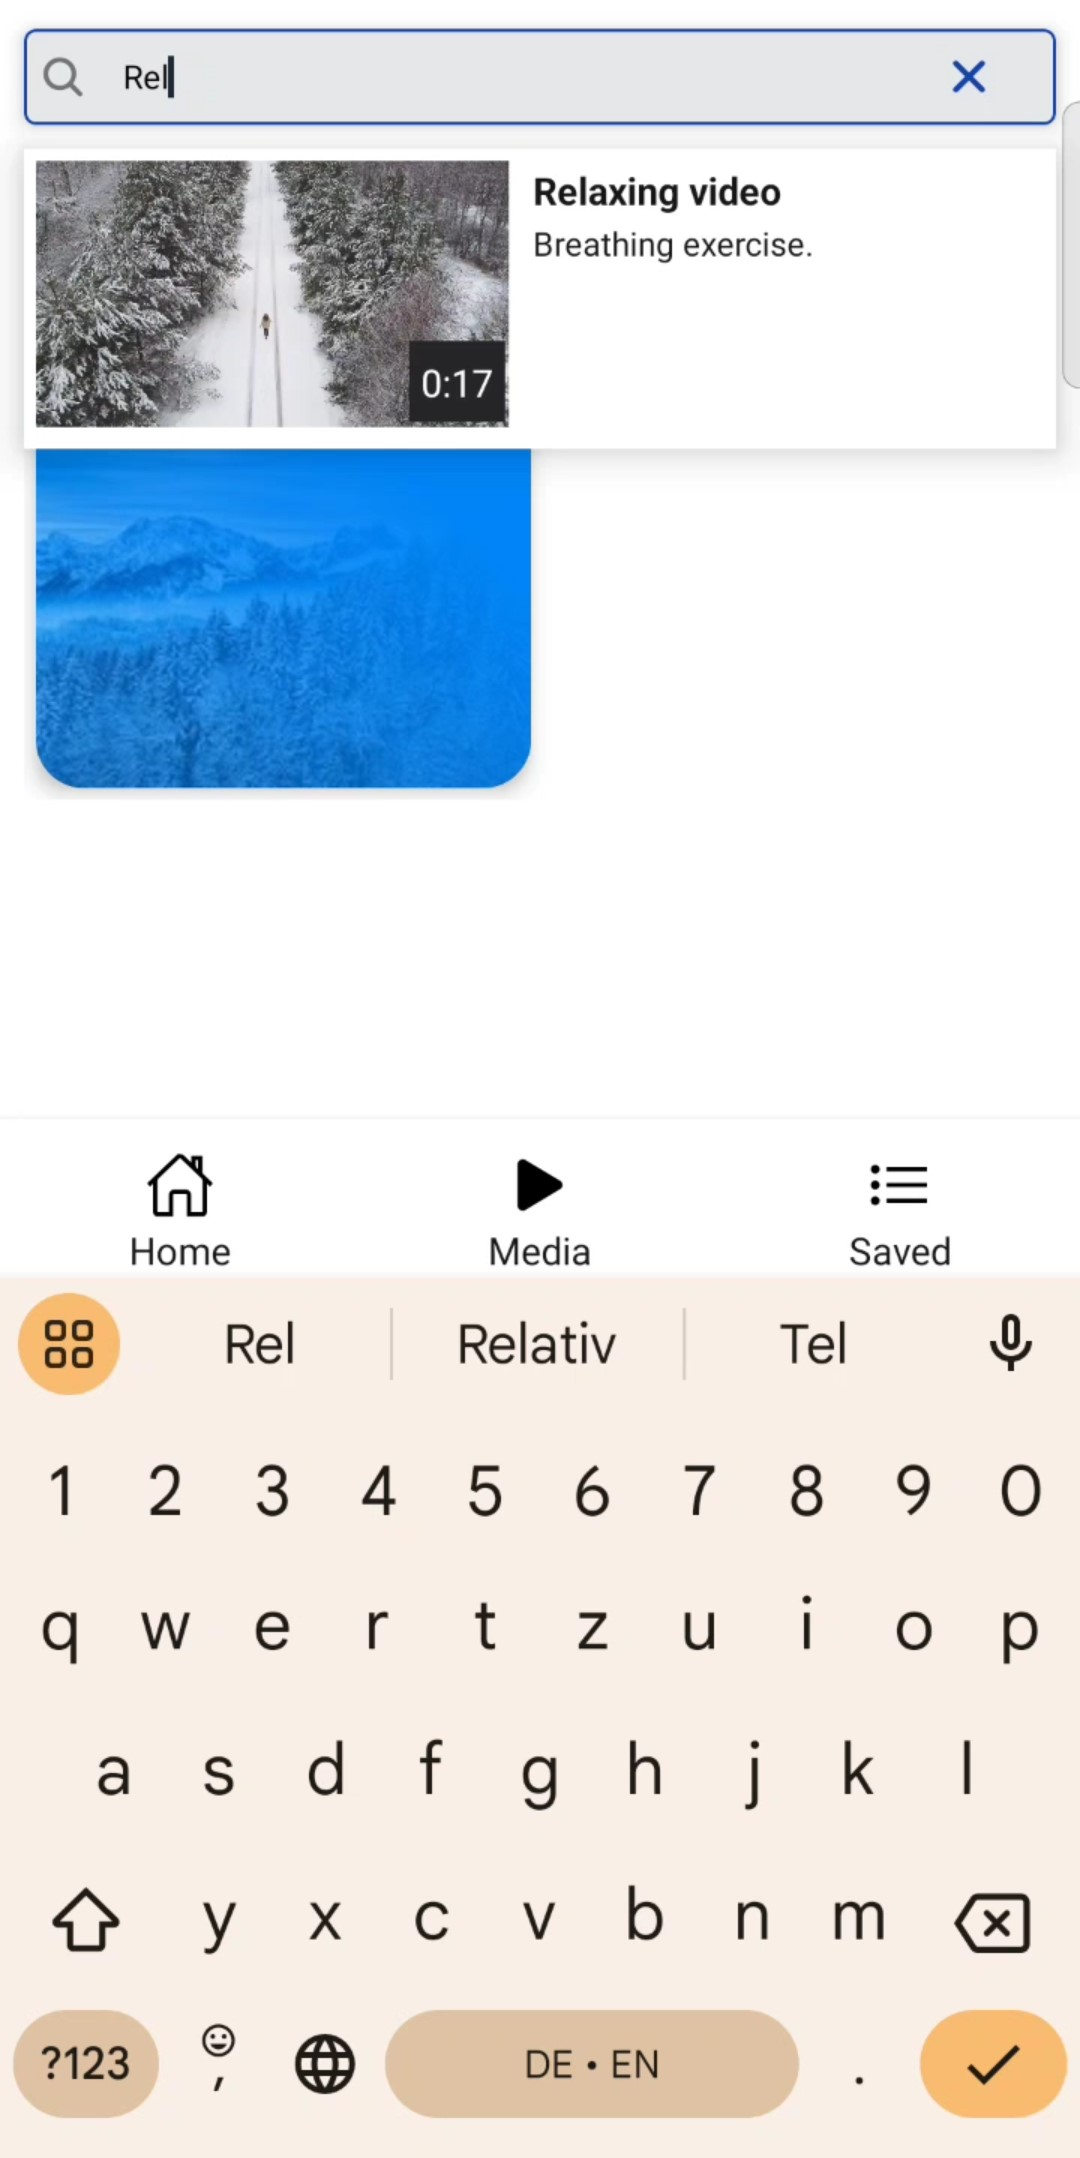
\includegraphics[height=\textwidth]{./pics/Suche.jpg}
    \caption{Suchleiste}
\end{figure}

\section{Media Player}

\begin{figure}[H]
    \begin{minipage}{0.5\textwidth}
        \centering
        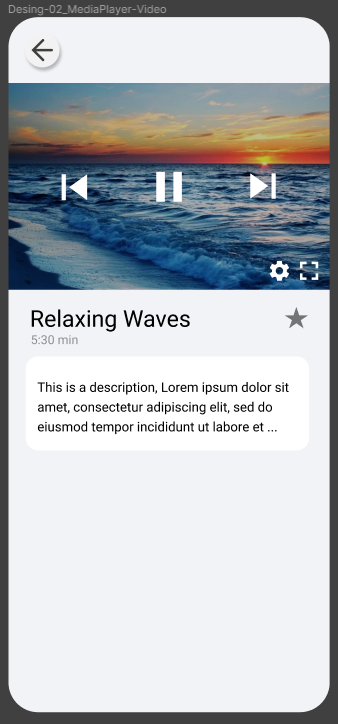
\includegraphics[height=2\textwidth]{./pics/pMediaPlayer.png}
        \caption{Media Player UI-Prototyp}
    \end{minipage}
    \begin{minipage}{0.5\textwidth}
        \centering
        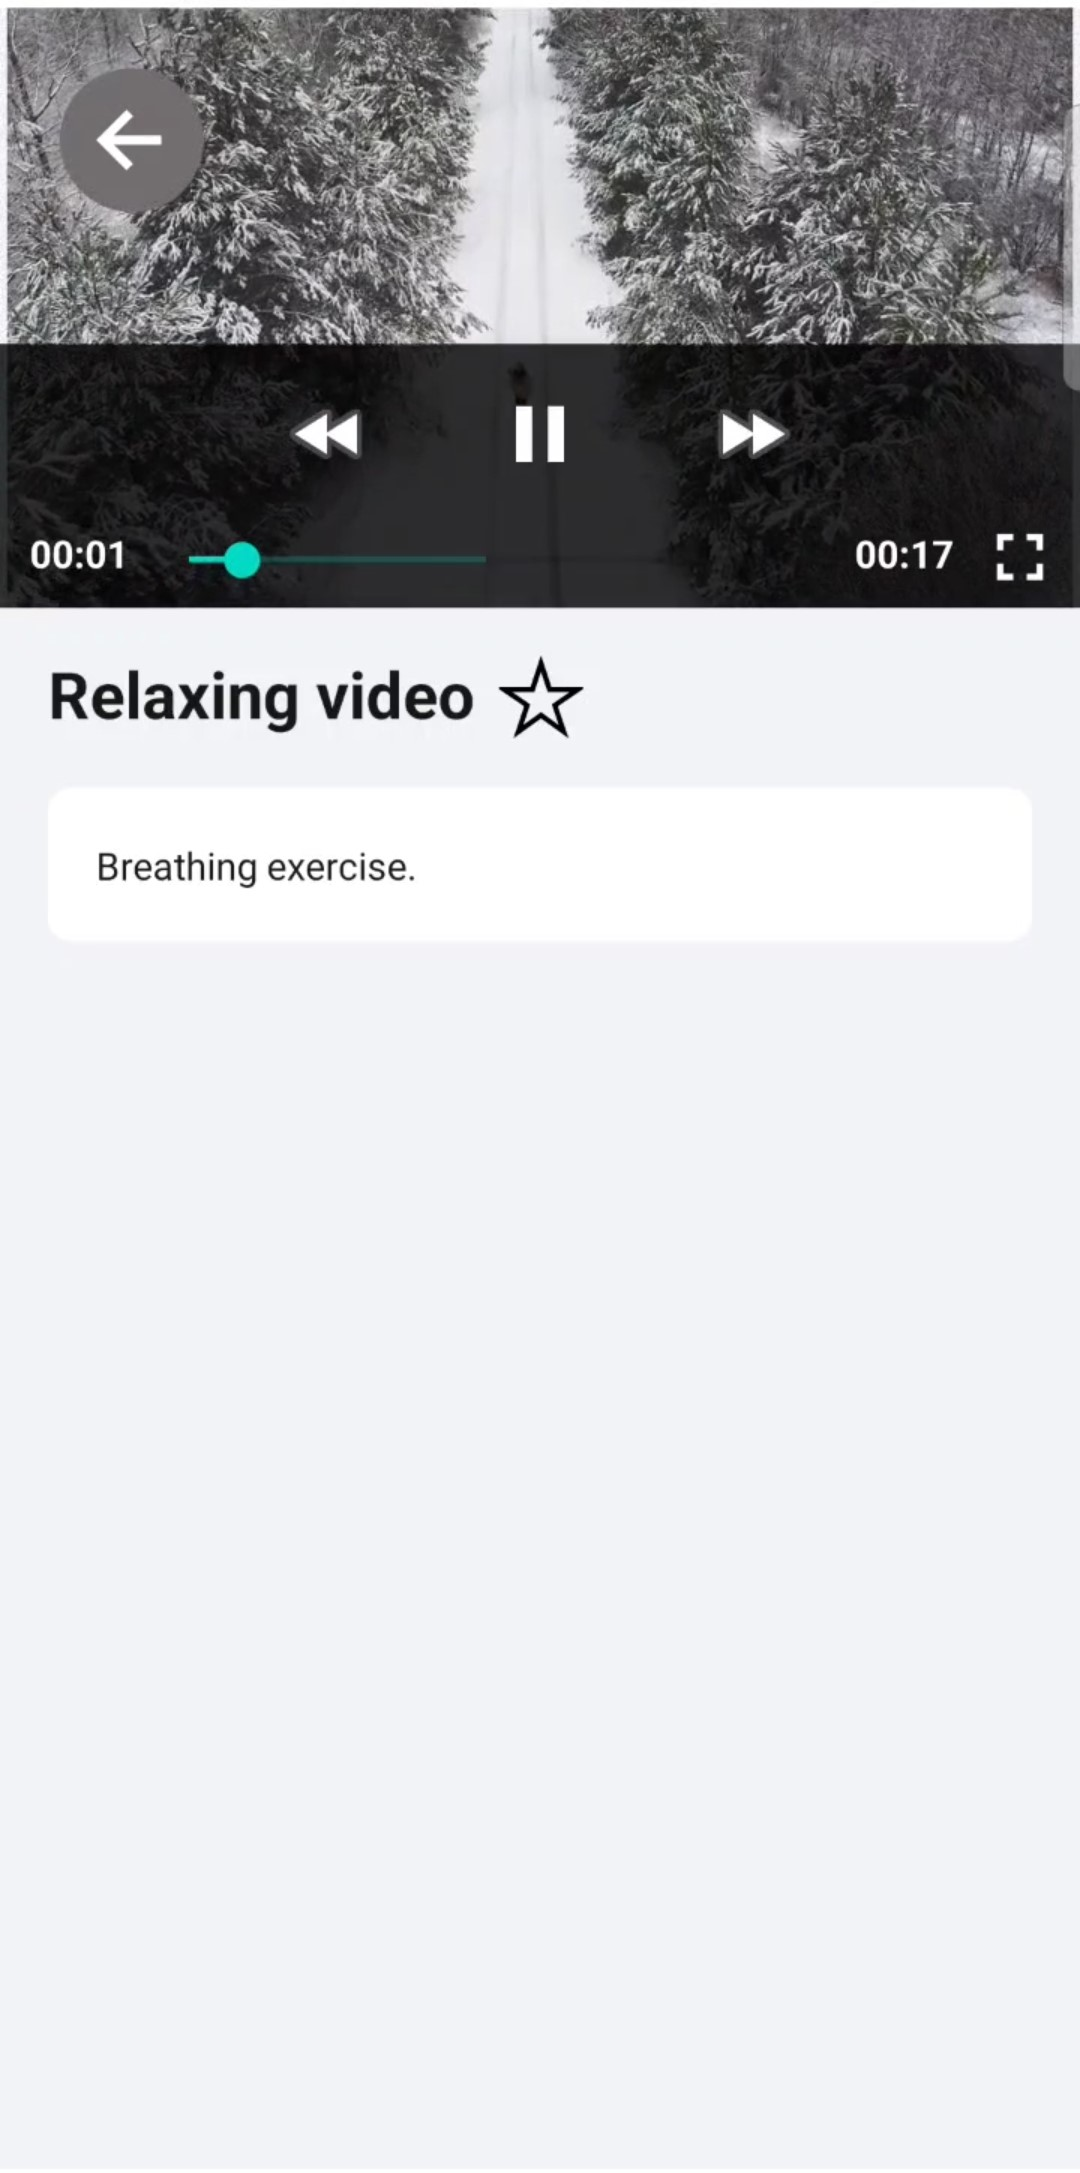
\includegraphics[height=2\textwidth]{./pics/MediaPlayer.jpg}
        \caption{Media Player in der App}
    \end{minipage}
\end{figure}

\section{Favoriten}

\begin{figure}[H]
    \centering
    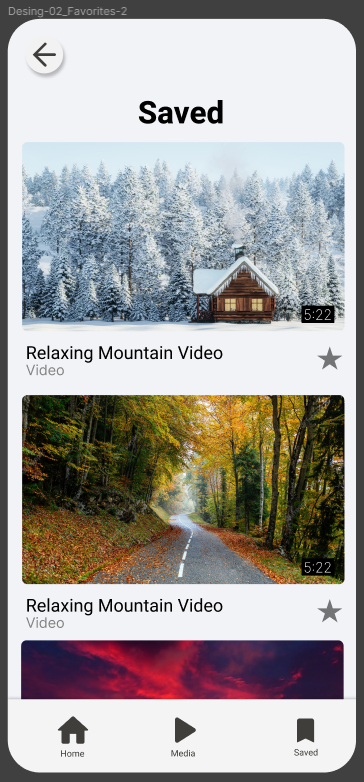
\includegraphics[height=\textwidth]{./pics/pFavoriten.png}
    \caption{Favoriten UI-Prototyp}
\end{figure}

\begin{figure}[H]
    \begin{minipage}{0.5\textwidth}
        \centering
        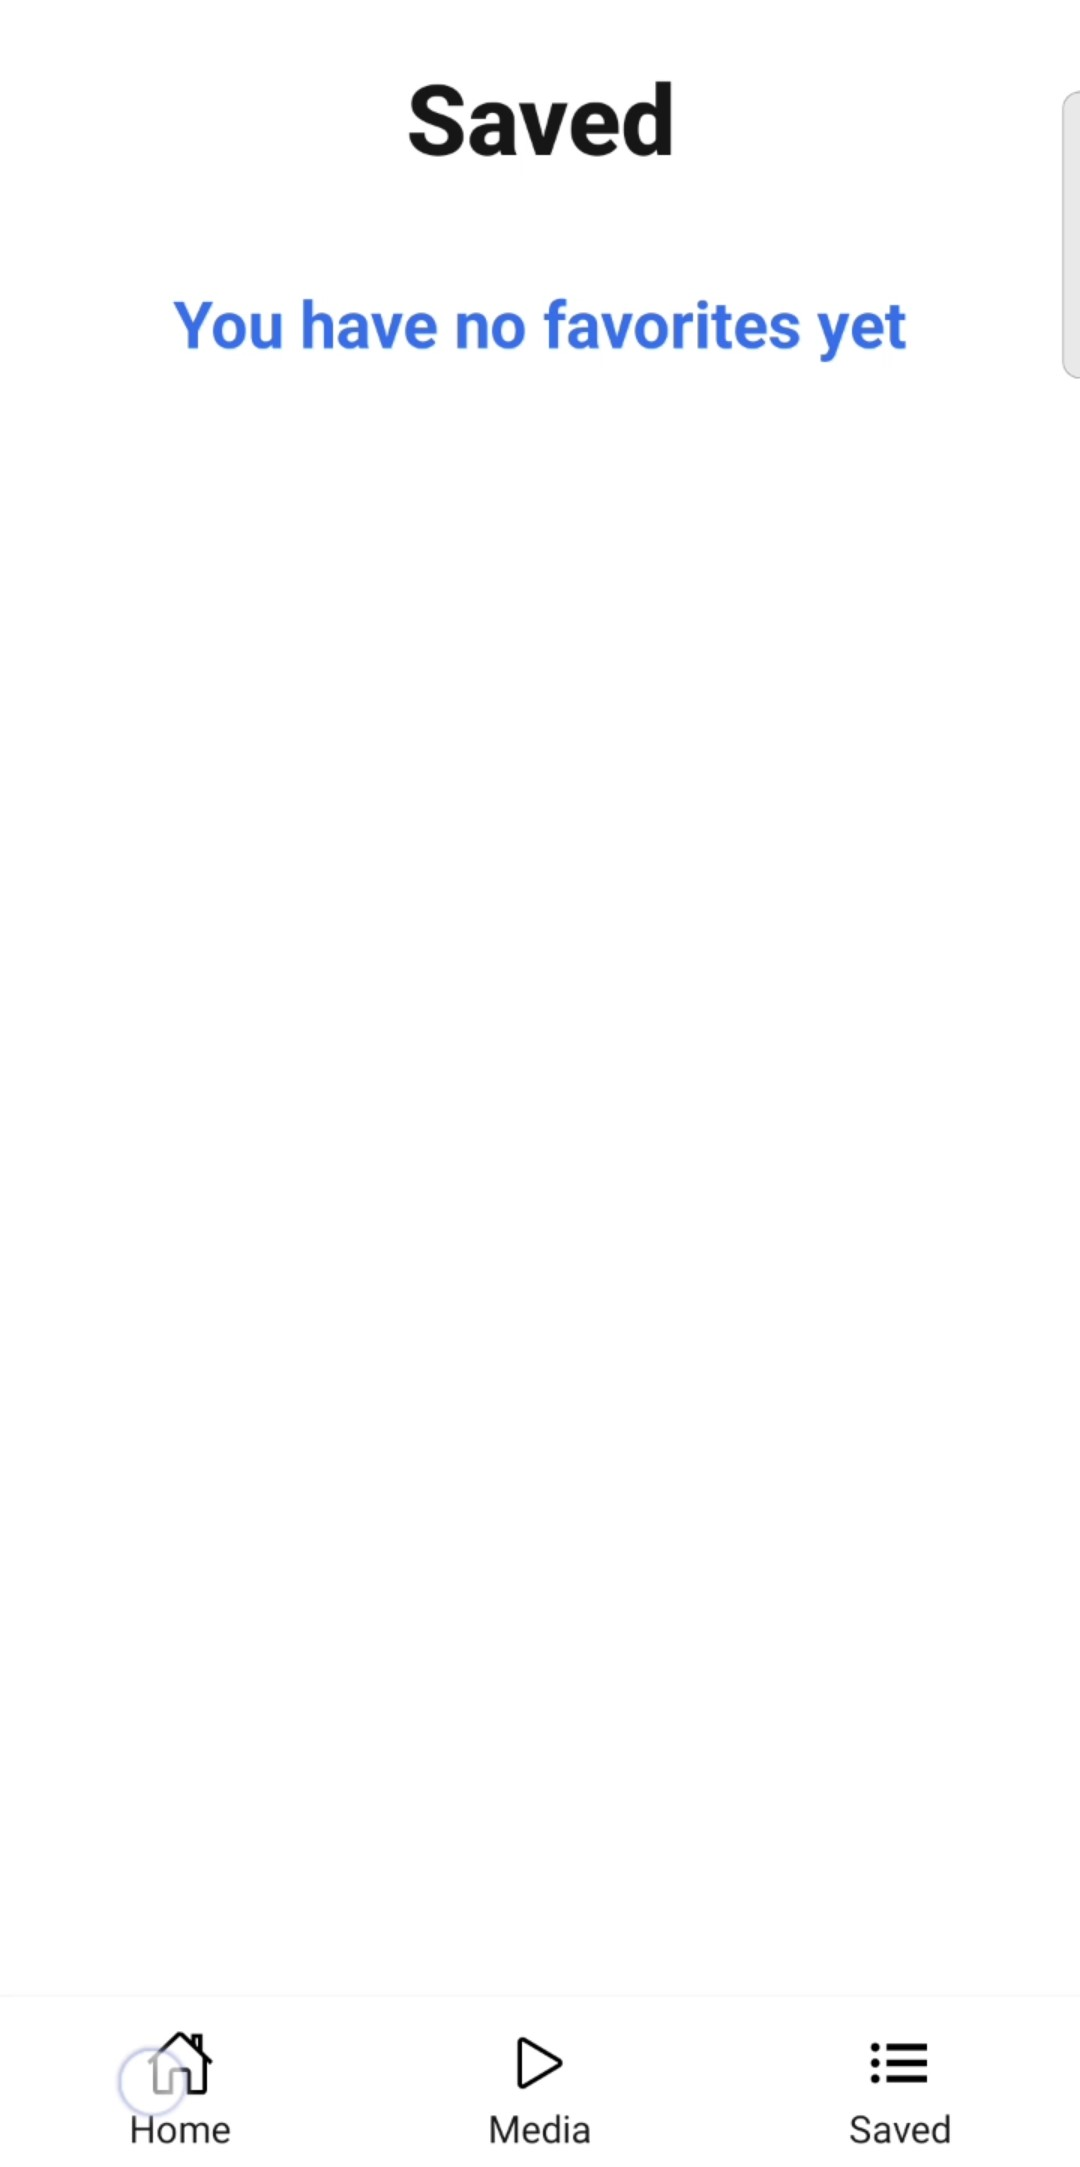
\includegraphics[height=2\textwidth]{./pics/No Favoriten.jpg}
        \caption{Kein Favorit gesetzt}
    \end{minipage}
    \begin{minipage}{0.5\textwidth}
        \centering
        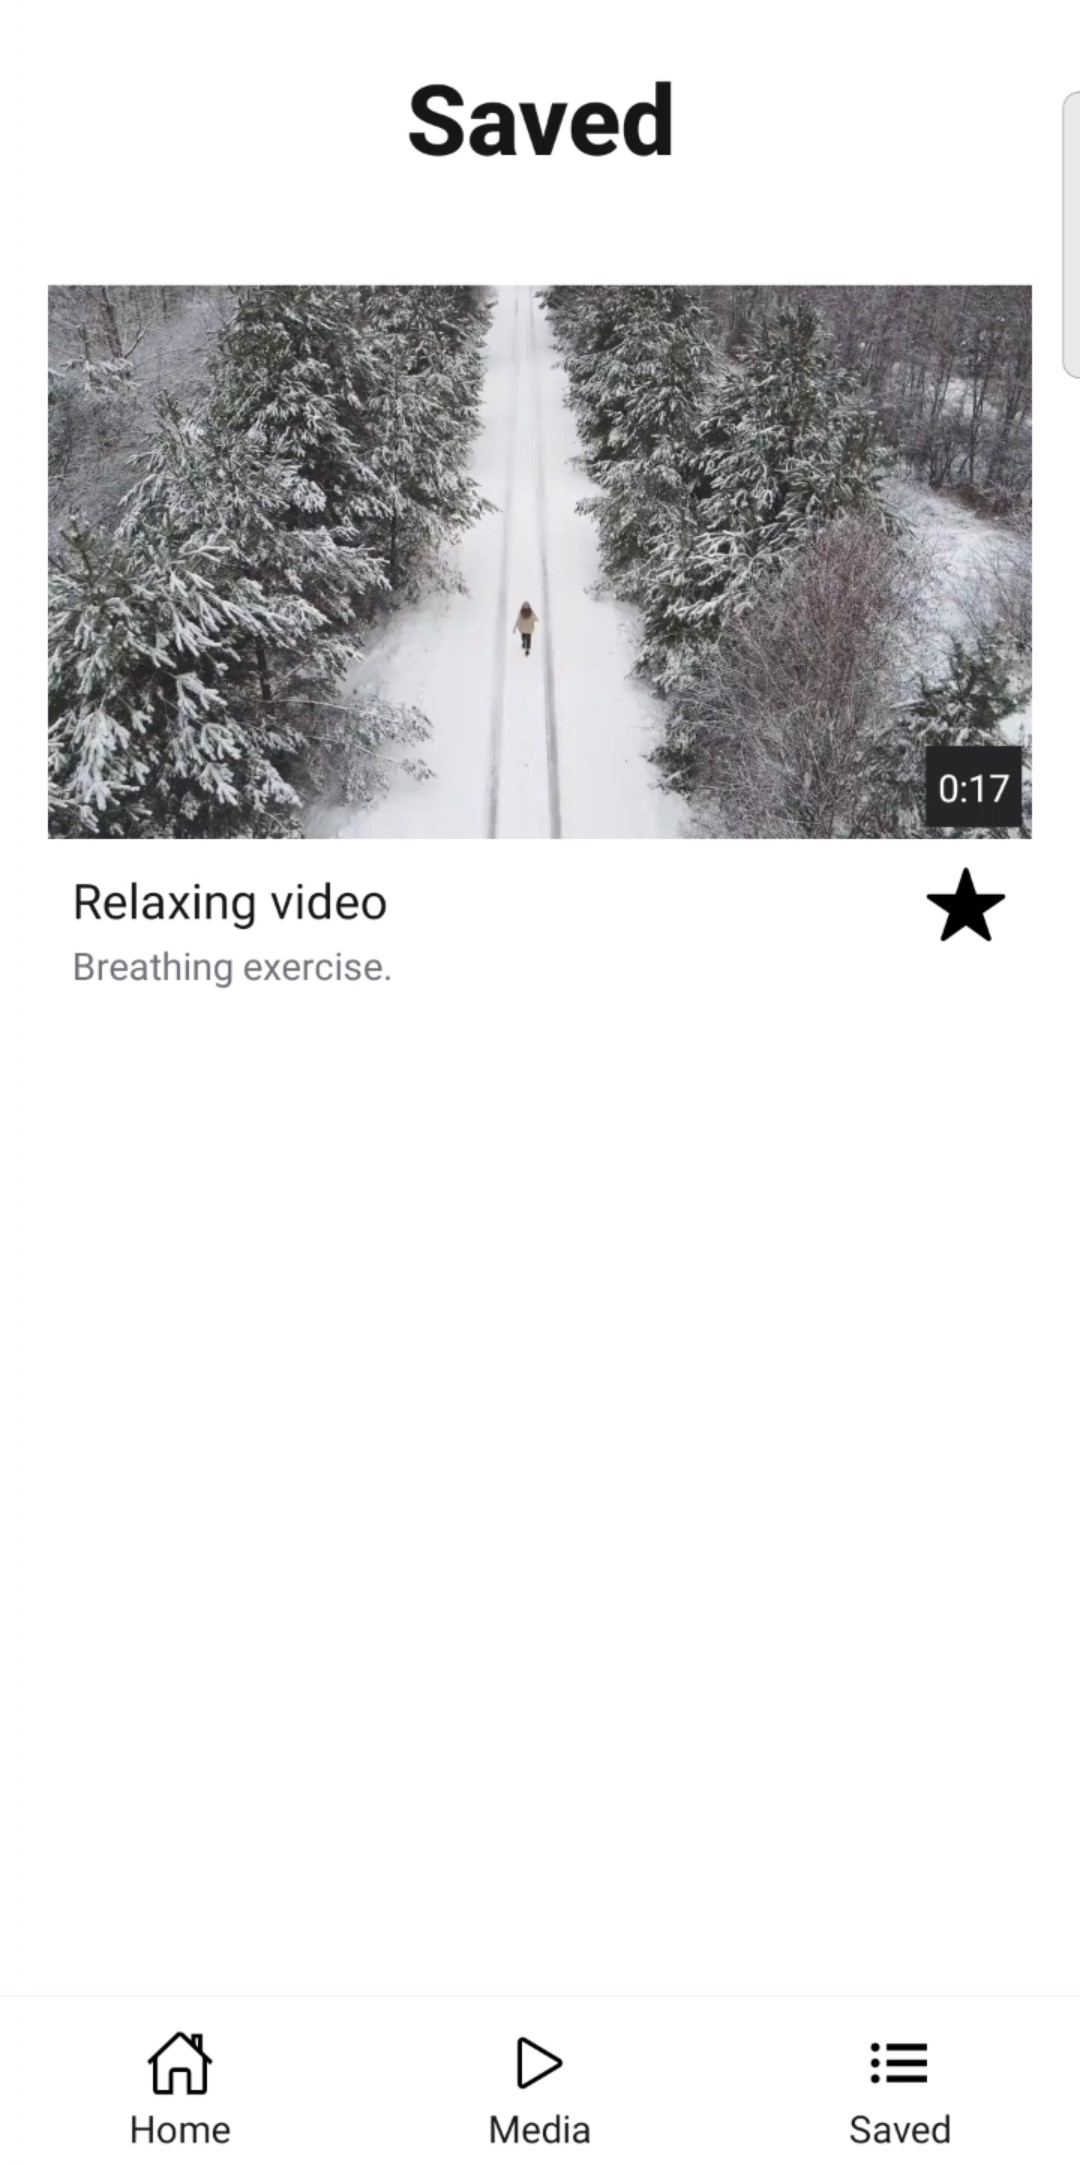
\includegraphics[height=2\textwidth]{./pics/Favoriten.jpg}
        \caption{Ein Favorit gesetzt}
    \end{minipage}
\end{figure}

\section{Einstellungen}

\begin{figure}[H]
    \centering
    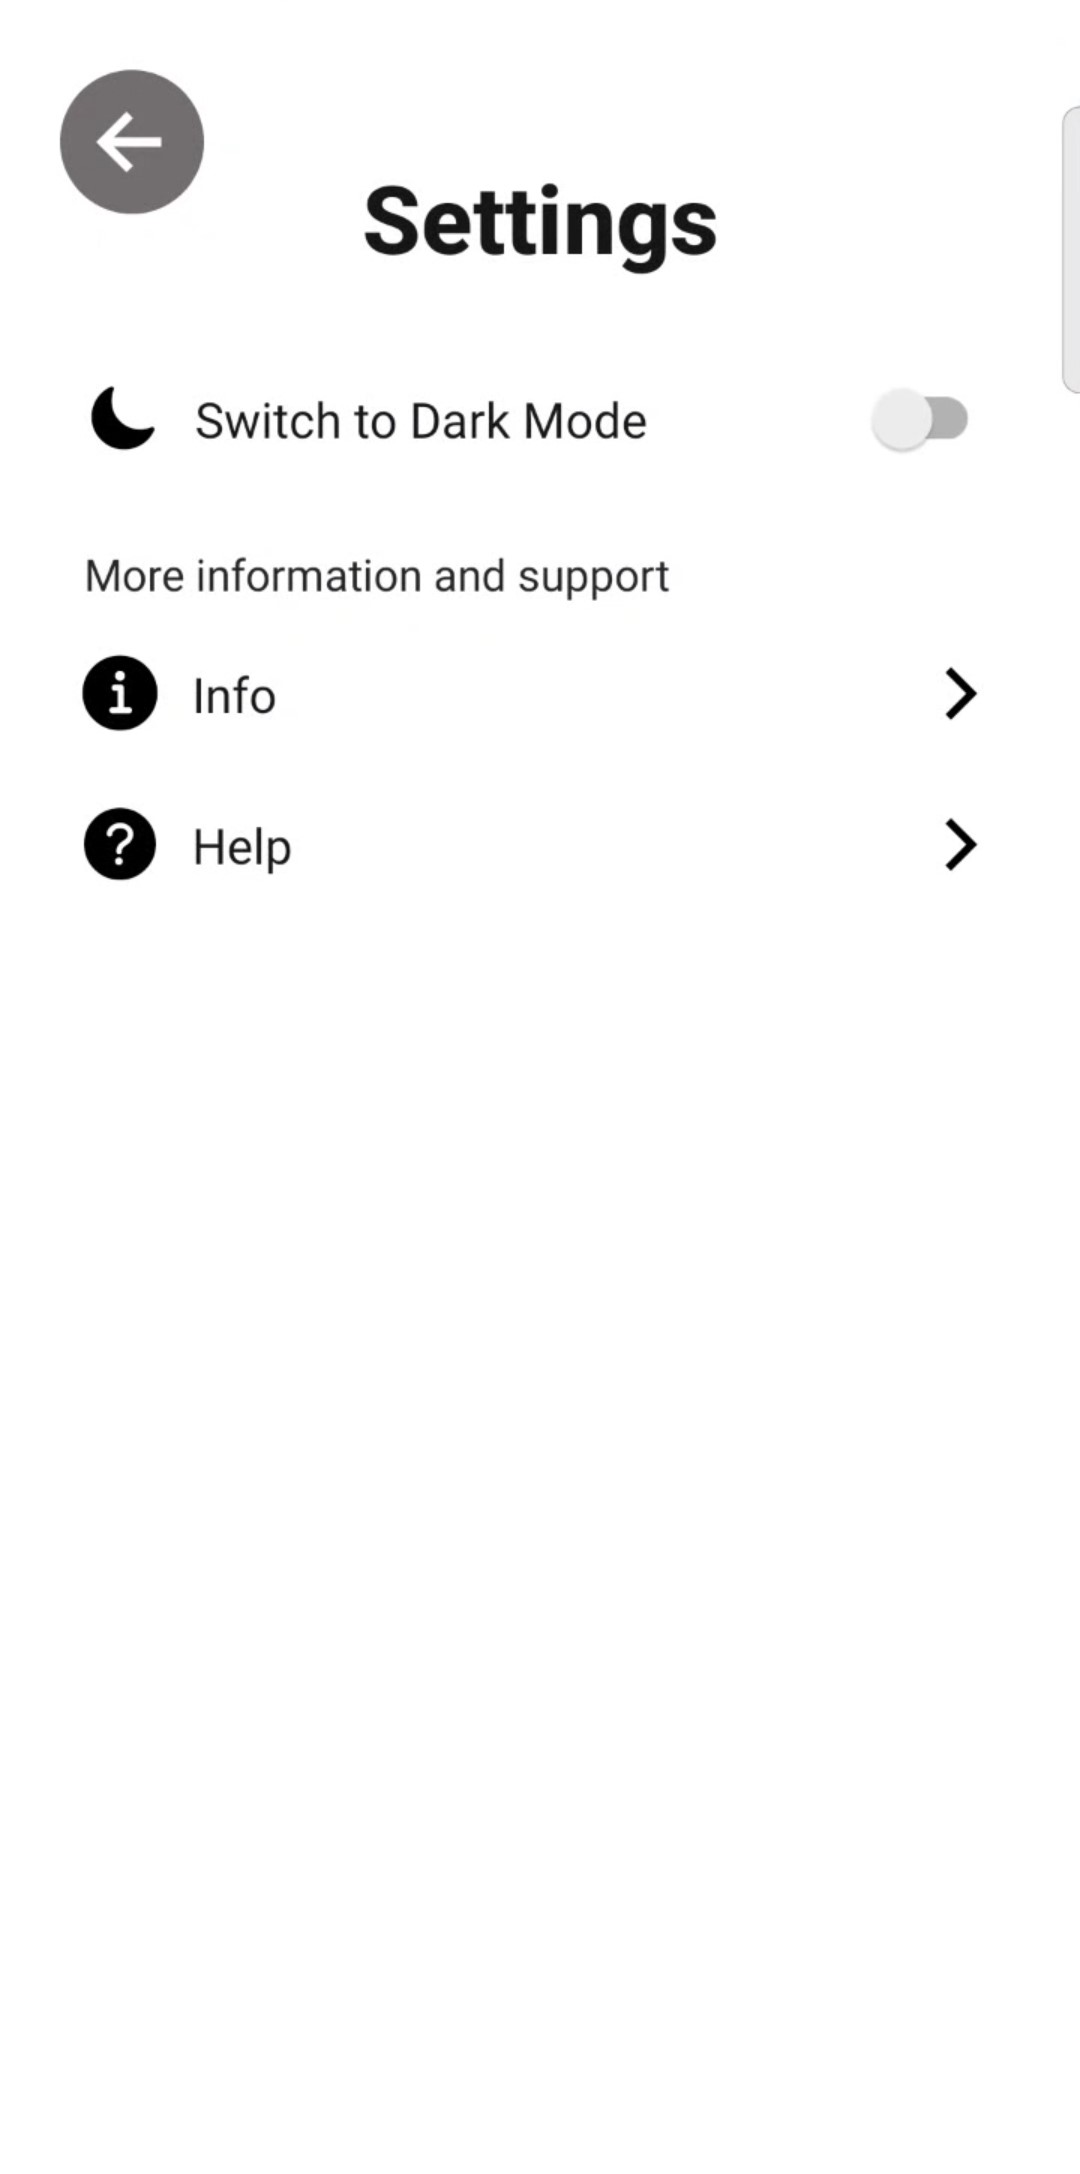
\includegraphics[height=\textwidth]{./pics/Settings.jpg}
    \caption{Einstellungen in der App}
\end{figure}

\section{Light/Dark Mode}

\begin{figure}[H]
    \begin{minipage}{0.5\textwidth}
        \centering
        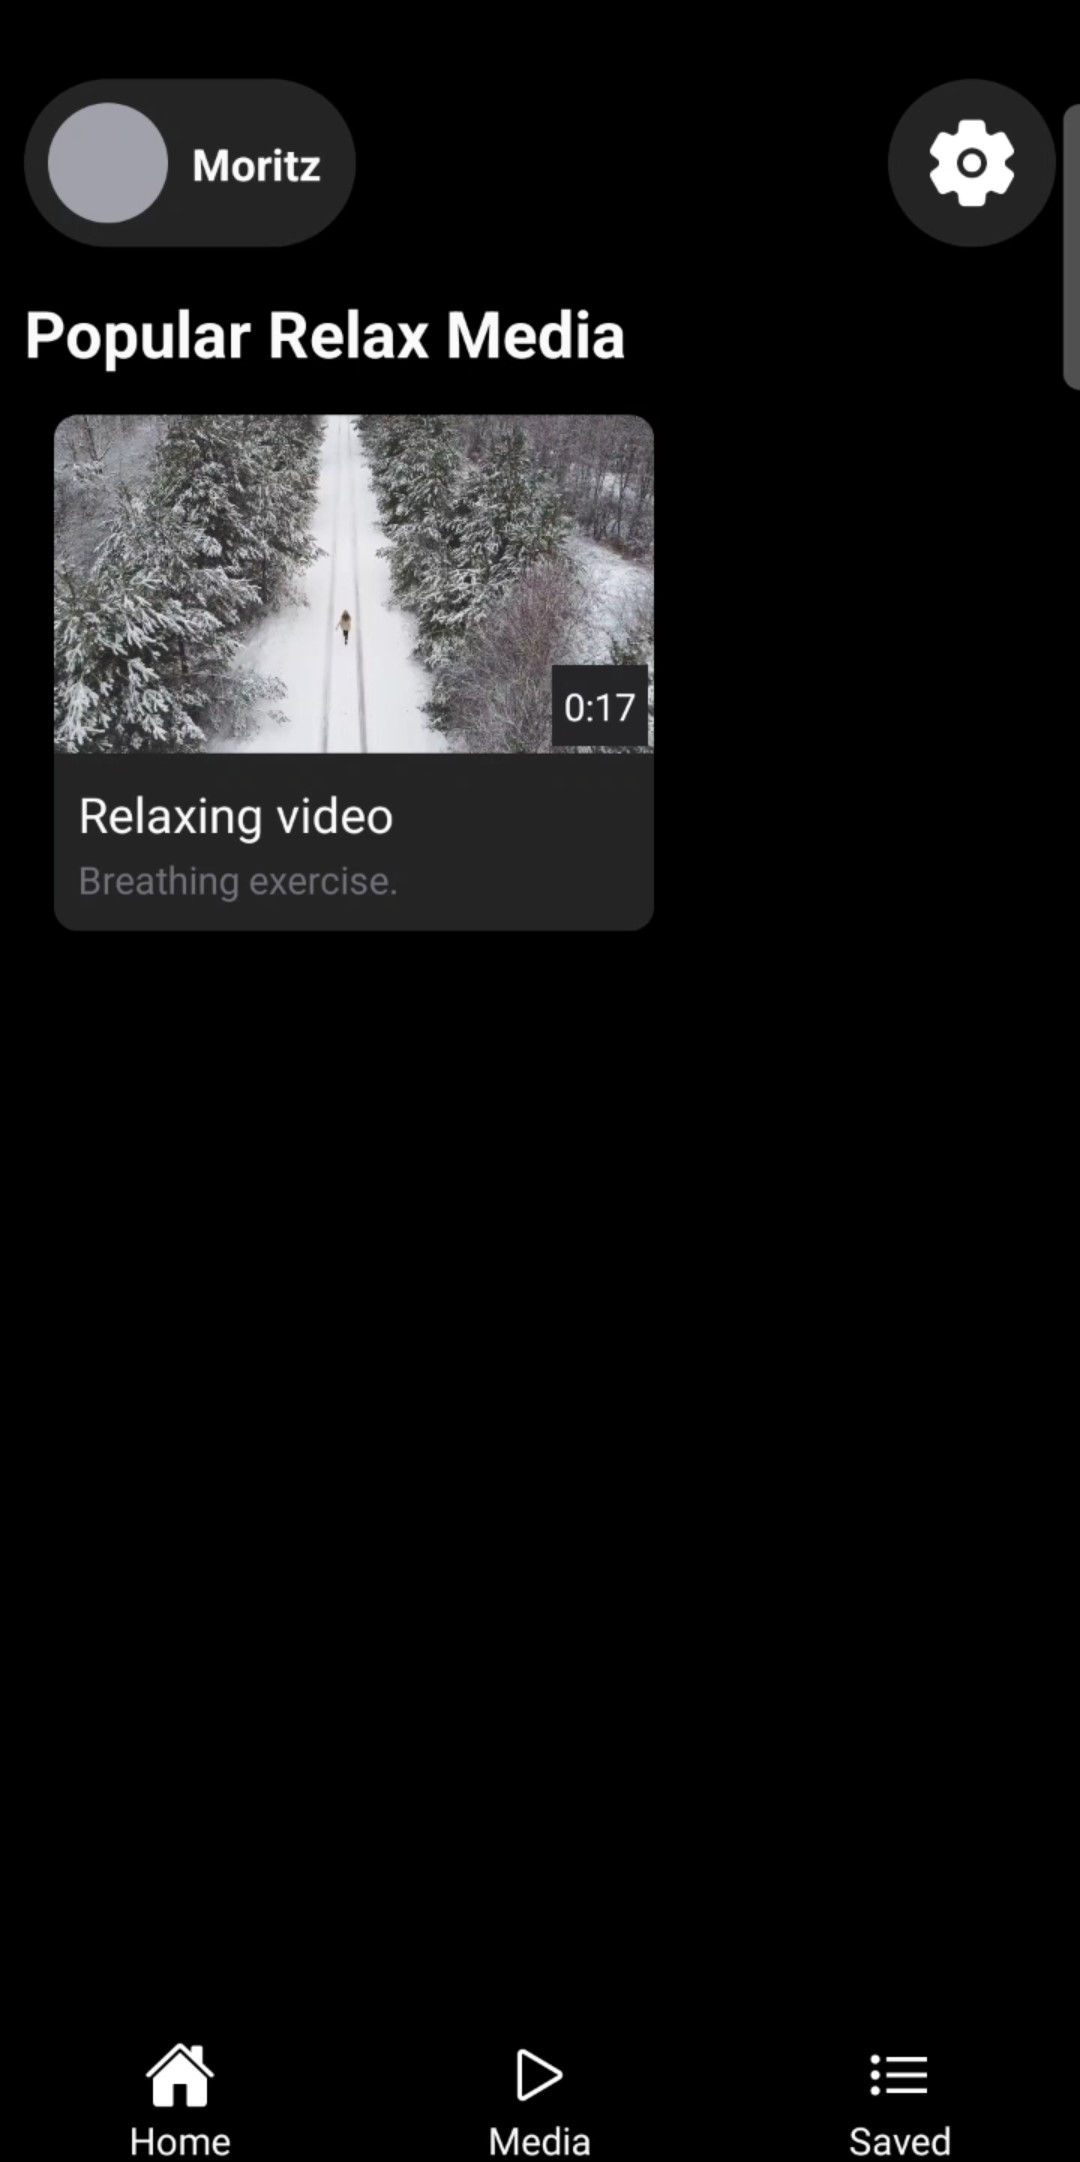
\includegraphics[height=1.4\textwidth]{./pics/dHome.jpg}
        \caption{Dark Home-Screen}
    \end{minipage}
    \begin{minipage}{0.5\textwidth}
        \centering
        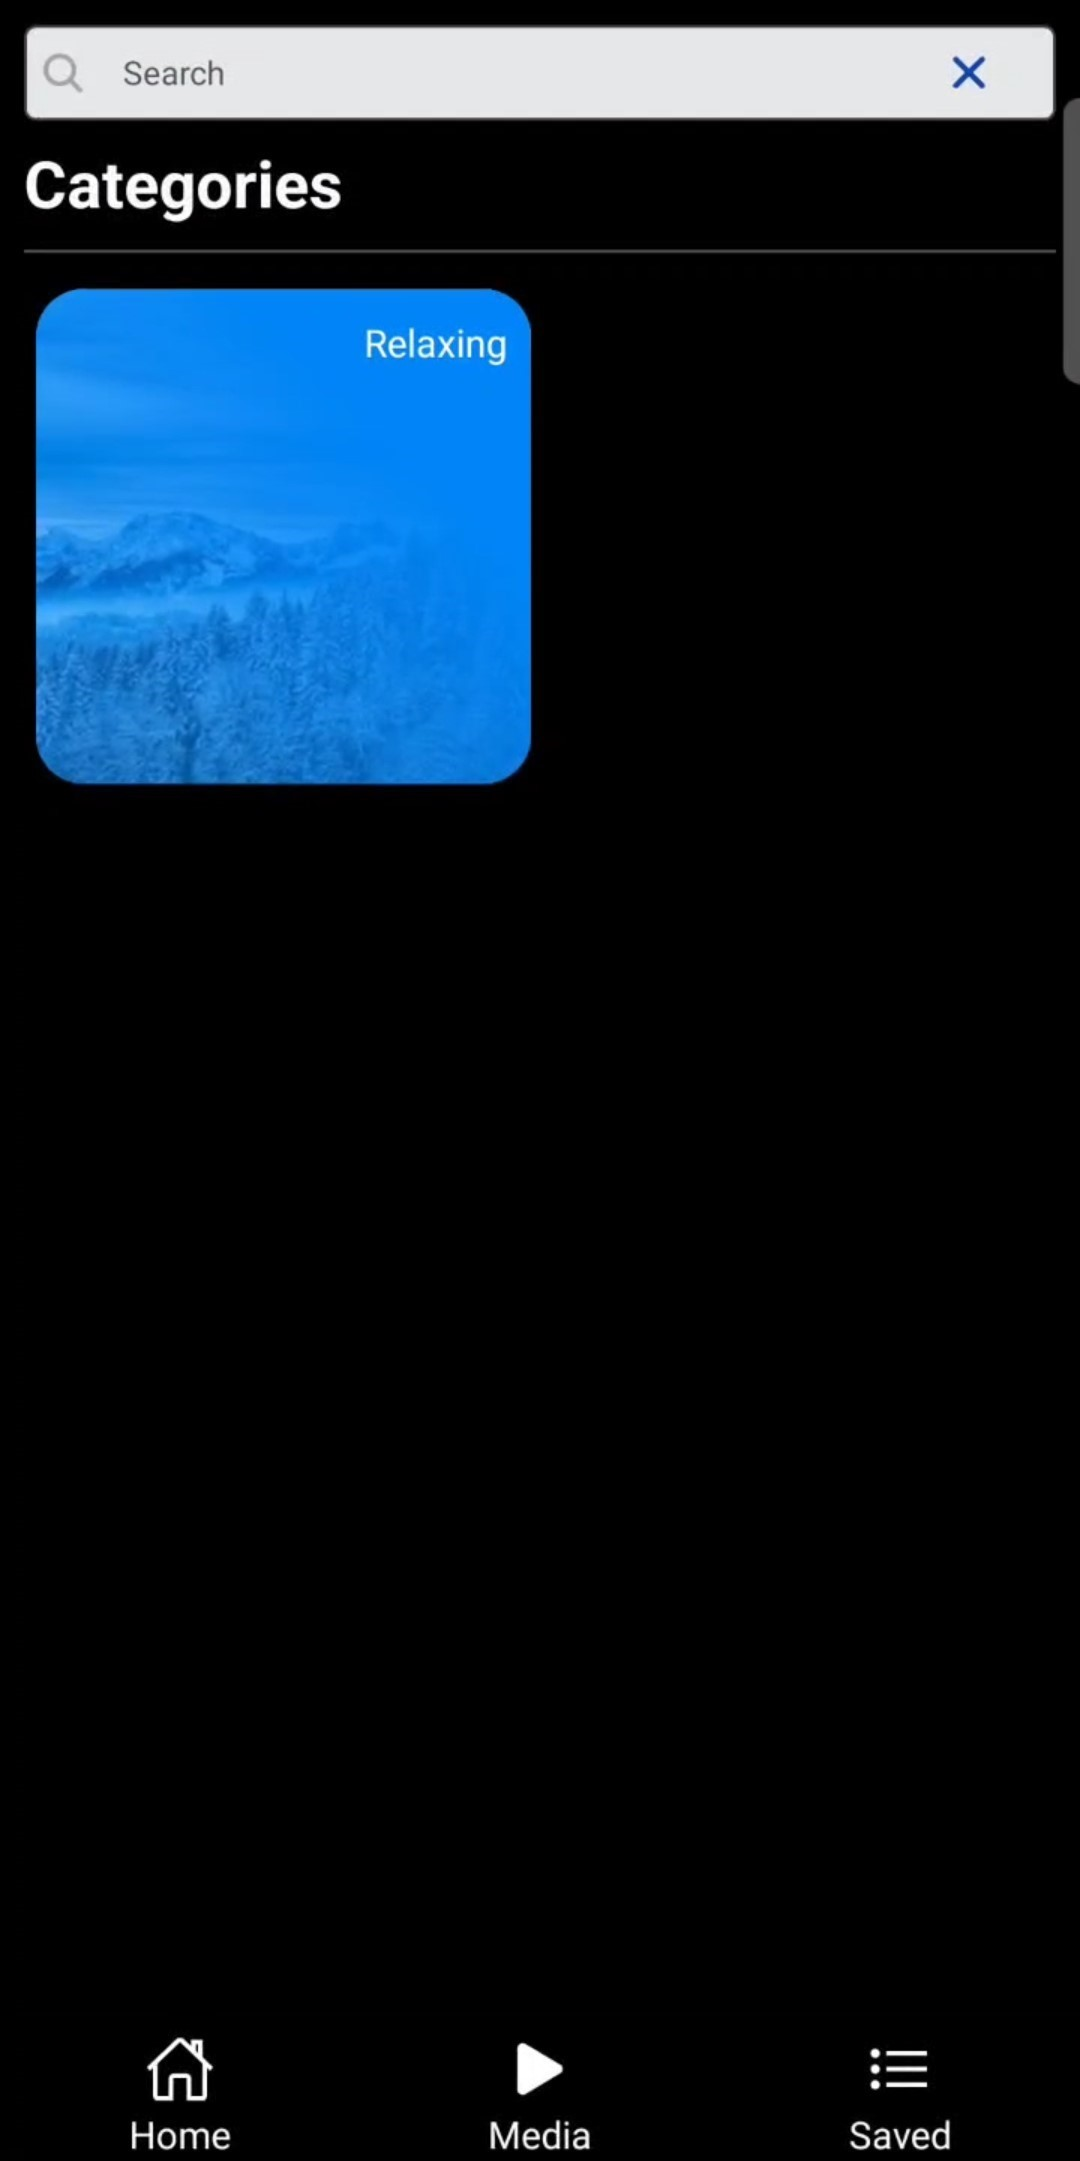
\includegraphics[height=1.4\textwidth]{./pics/dKategorie.jpg}
        \caption{Dark Kategorie-Screen}
    \end{minipage}
\end{figure}
\begin{figure}[H]
    \begin{minipage}{0.5\textwidth}
        \centering
        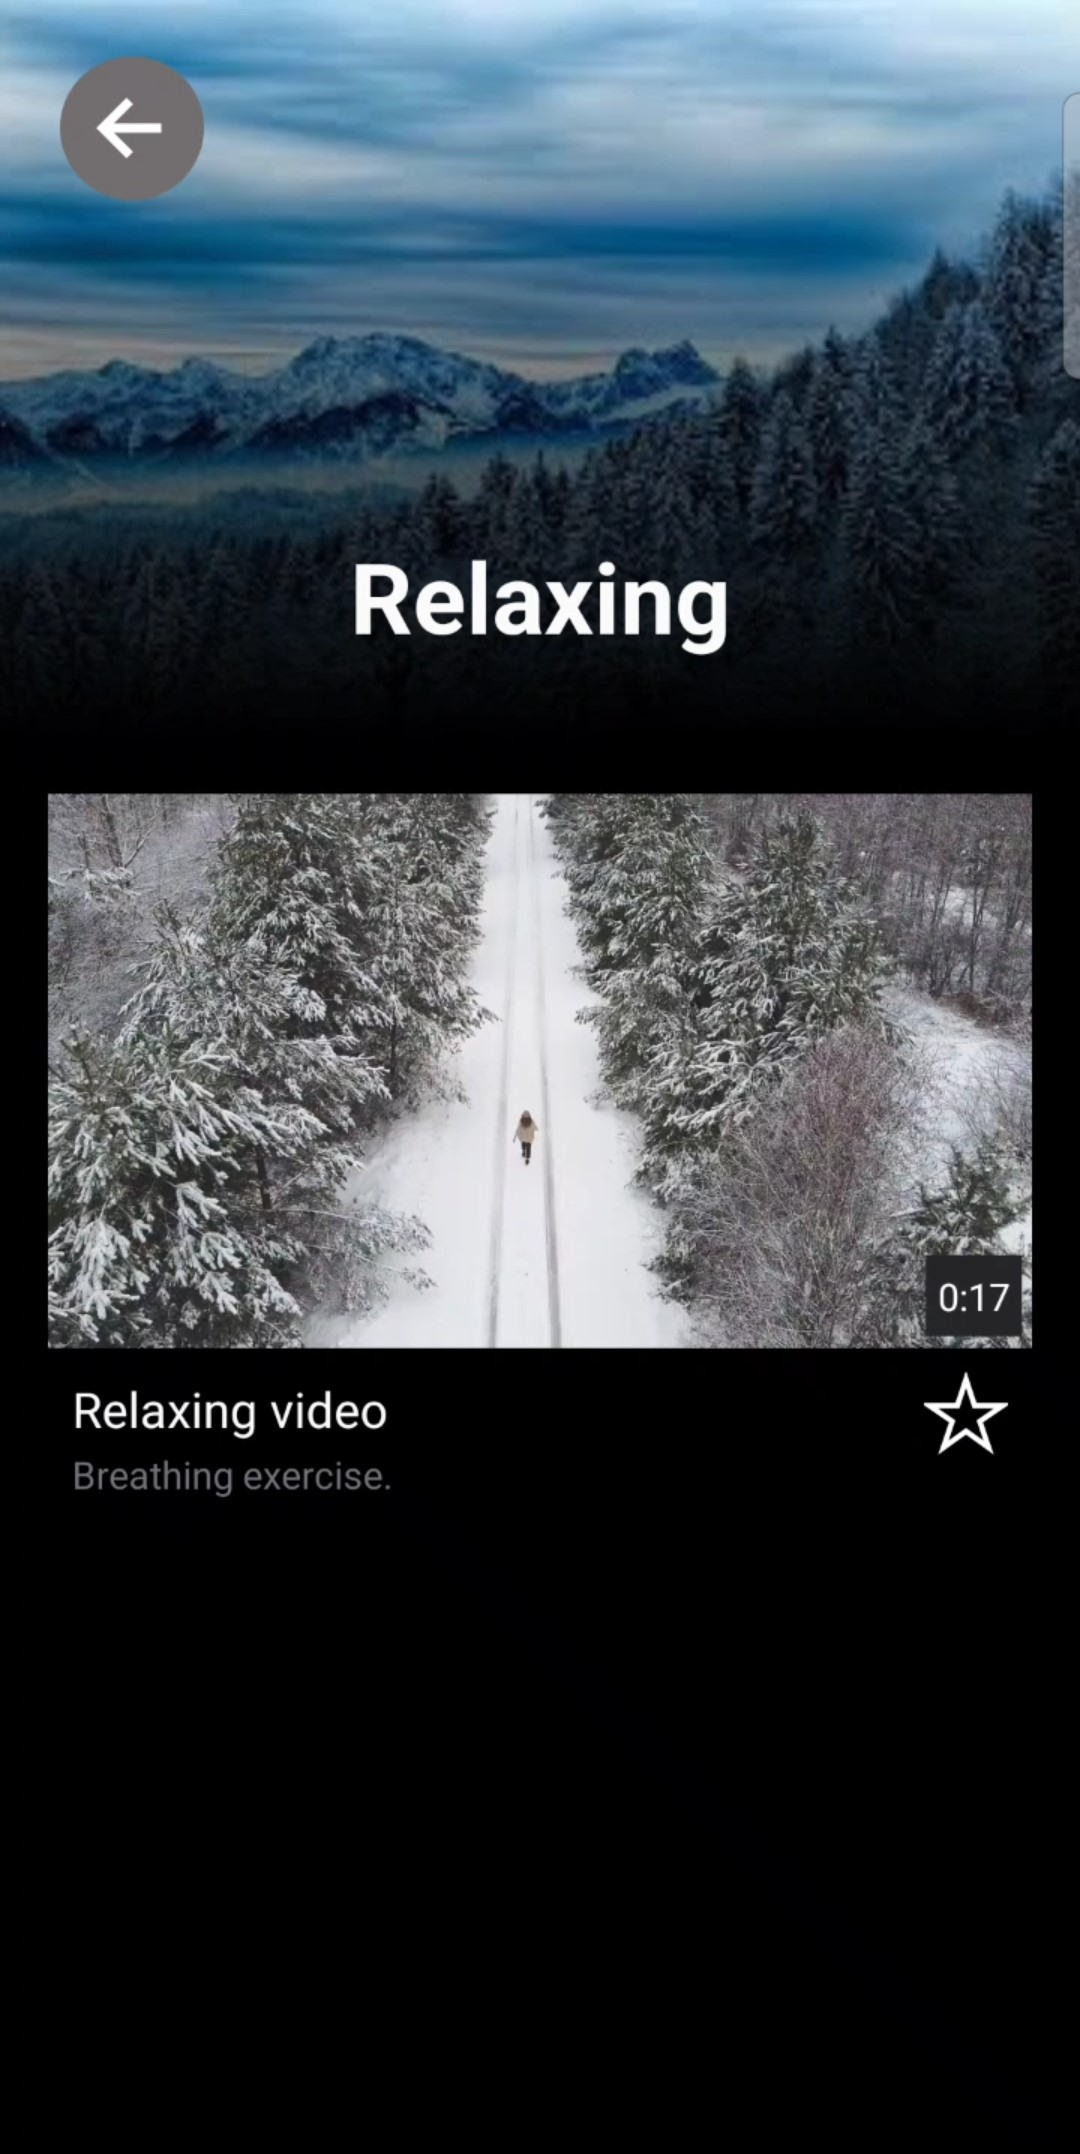
\includegraphics[height=1.4\textwidth]{./pics/dMedia.jpg}
        \caption{Dark Media-Screen}
    \end{minipage}
    \begin{minipage}{0.5\textwidth}
        \centering
        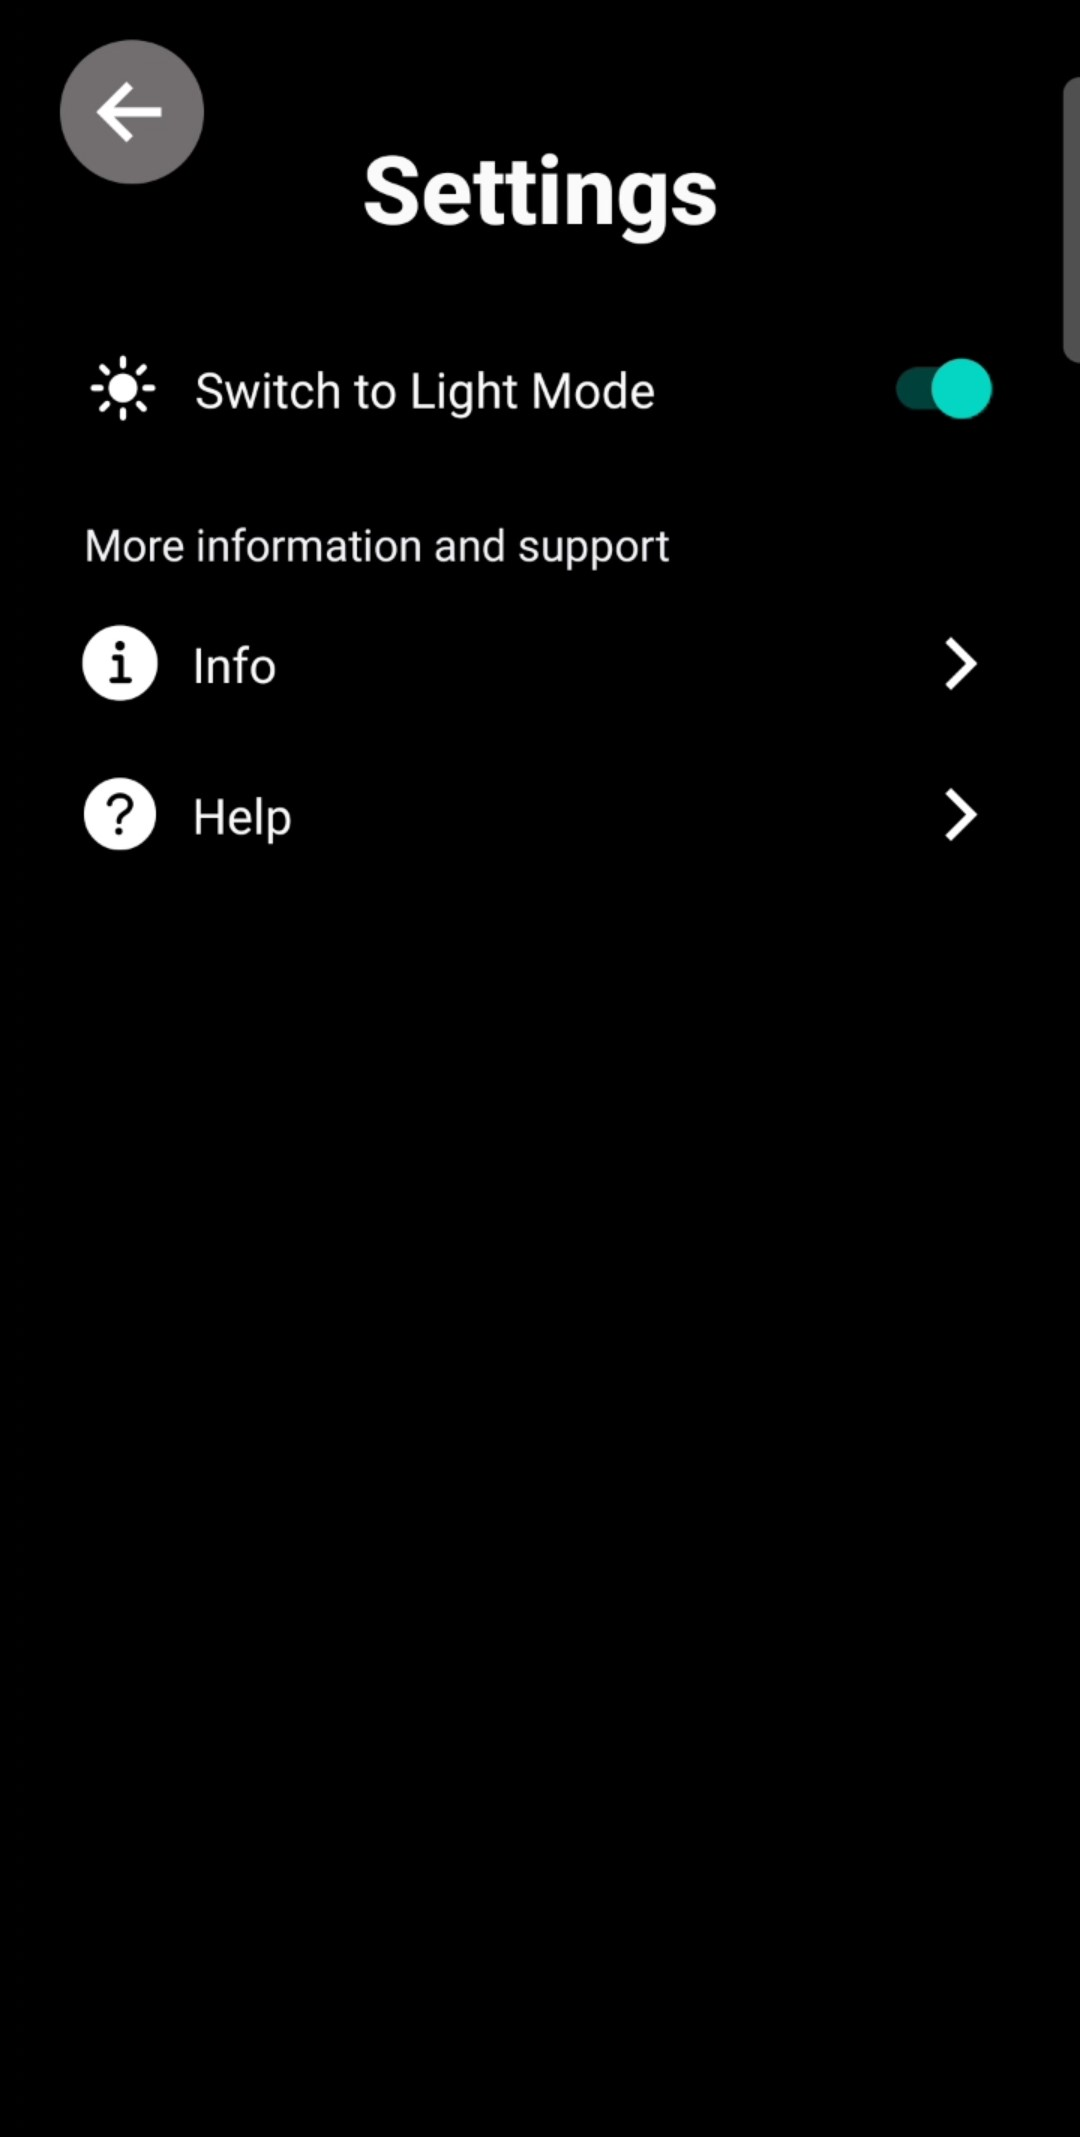
\includegraphics[height=1.4\textwidth]{./pics/dSettings.jpg}
        \caption{Dark Settings-Screen}
    \end{minipage}
\end{figure}

\section{Logo}

\begin{figure}[H]
    \begin{minipage}{0.5\textwidth}
        \centering
        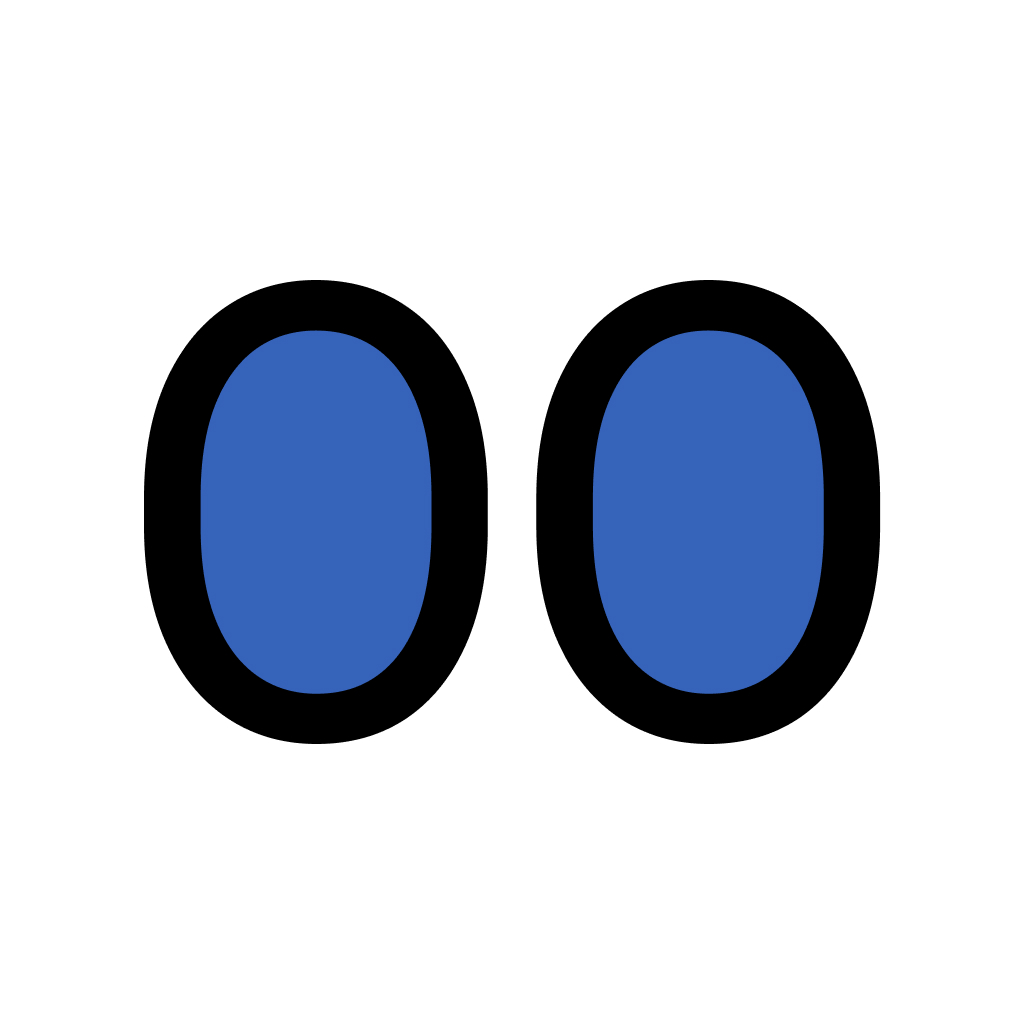
\includegraphics[height=0.6\textwidth]{./pics/Relaxoon Logo White.jpg}
        \caption{Logo white}
    \end{minipage}
    \begin{minipage}{0.5\textwidth}
        \centering
        
\includegraphics[height=0.6\textwidth]{./pics/Relaxoon Logo Black.jpg}
        \caption{Logo black}
    \end{minipage}
\end{figure}